\documentclass[12pt,a4paper]{article}

% Informe Final del proyecto KIWI para el curso de DevOps (IS4024).
% Integra el informe parcial (arquitectura, Git, pruebas, Bash y Docker) con
% los requisitos a-m de "Proyecto - Informe final.pdf": modelo STRIDE
% (diagramas/STRIDE.drawio), pipeline DevSecOps, DefectDojo, monitoreo,
% madurez, lecciones y recomendaciones. Cifras tomadas de
% docs/devsecops/cierre y de los artefactos de CI citados en el texto.

\usepackage[utf8]{inputenc}
\usepackage[T1]{fontenc}
\usepackage{lmodern}
\usepackage[nopatch=footnote]{microtype}
\usepackage[spanish,provide=*]{babel}
\usepackage{geometry}
\geometry{margin=2.5cm,headheight=14pt}

\usepackage{graphicx}
\usepackage{xcolor}
\usepackage{hyperref}
\usepackage{tocloft}
\usepackage{booktabs,array,tabularx}
\usepackage{amsmath,amssymb}
\usepackage{enumitem}
\usepackage{fancyhdr}
\usepackage{float}
\usepackage[section]{placeins}
\usepackage{caption,subcaption}
\usepackage{listings}
\usepackage{xurl}
\usepackage{seqsplit}
\usepackage{tikz}
\usetikzlibrary{positioning,arrows.meta,shapes.geometric}
\usepackage{longtable}
\usepackage{pdflscape}

\setlength{\parindent}{0pt}
\setlength{\parskip}{4pt}
\setlength{\emergencystretch}{2em}

% Columnas con texto alineado a la izquierda. Se definen en el preambulo para
% que el caracter > no dependa de los atajos de babel dentro del documento.
\newcolumntype{L}[1]{>{\raggedright\arraybackslash}p{#1}}
\newcolumntype{Y}{>{\raggedright\arraybackslash}X}

% Rutas de archivos del repositorio: tipografia monoespaciada y corte de linea
% en cualquier caracter (xurl), tambien dentro de captions y tablas.
\DeclareRobustCommand{\ruta}[1]{\nolinkurl{#1}}

\definecolor{utecblue}{RGB}{0,70,127}
\definecolor{lightgray}{RGB}{245,245,245}
\definecolor{pendingborder}{RGB}{150,150,150}

% Enlaces internos en negro (citas, referencias cruzadas, indice) para que el
% documento impreso se vea sobrio; solo las URL de la bibliografia van en color,
% porque ahi el color si comunica que el enlace es accionable.
\hypersetup{
  colorlinks=true,
  linkcolor=black,
  citecolor=black,
  urlcolor=utecblue
}

\renewcommand{\cftsecleader}{\cftdotfill{\cftdotsep}}
% Indice compacto: con las secciones y subsecciones que tiene el informe, el
% espaciado por defecto lo desborda a una segunda pagina casi vacia.
\setlength{\cftbeforesecskip}{0pt}
\setlength{\cftbeforesubsecskip}{0pt}
\captionsetup[figure]{labelfont=bf,font=small}
\captionsetup[table]{labelfont=bf,font=small}
\graphicspath{{images/}}

\lstset{
  basicstyle=\ttfamily\small,
  backgroundcolor=\color{lightgray},
  frame=single,
  rulecolor=\color{gray},
  framerule=0.6pt,
  breaklines=true,
  columns=fullflexible,
  keepspaces=true,
  tabsize=4,
  numbers=left,
  numberstyle=\tiny\color{gray},
  xleftmargin=8pt,
  xrightmargin=8pt,
  captionpos=b
}

% Estilo para el anexo con el workflow completo: letra menor y acentos de los
% comentarios del YAML convertidos a comandos LaTeX.
\lstdefinestyle{yaml}{
  basicstyle=\ttfamily\scriptsize,
  numberstyle=\tiny\color{gray},
  breakatwhitespace=false,
  literate={á}{{\'a}}1 {é}{{\'e}}1 {í}{{\'i}}1 {ó}{{\'o}}1 {ú}{{\'u}}1
           {ñ}{{\~n}}1 {Á}{{\'A}}1 {É}{{\'E}}1 {Í}{{\'I}}1 {Ó}{{\'O}}1
           {Ú}{{\'U}}1 {Ñ}{{\~N}}1 {ü}{{\"u}}1 {·}{{$\cdot$}}1 {─}{{-}}1
}

\addto\captionsspanish{
  \renewcommand{\tablename}{Tabla}
  \renewcommand{\lstlistingname}{Código}
}

% Recuadro reutilizable para marcar donde va una captura de pantalla real
% (historial de commits, Pull Requests, ejecución de tests, contenedores
% corriendo) que debe insertarse a mano antes de la entrega final, porque
% este documento se genera sin acceso a la interfaz de GitHub ni a una
% terminal con el proyecto corriendo.
\newcommand{\capturaPendiente}[1]{%
  \begin{center}
  \fbox{\parbox{0.92\textwidth}{\centering\vspace{0.6cm}
  \textit{[Espacio reservado para captura de pantalla: #1]}
  \vspace{0.6cm}}}
  \end{center}
}

% Datos editables de portada.
\newcommand{\projectTitle}{KIWI}
\newcommand{\projectSubtitle}{Proyecto Informe Final}
\newcommand{\courseName}{DevOps}
\newcommand{\courseCode}{IS4024}
\newcommand{\professorName}{Wilson Julca Mejia}
\newcommand{\memberOne}{Aarón Timaná Castro}
\newcommand{\memberTwo}{Jean Piero Huaylla Huillca}
\newcommand{\memberThree}{Mateo Espinoza Monti}

\pagestyle{fancy}
\fancyhf{}
\fancyhead[L]{\small \courseCode{} -- \courseName}
\fancyhead[R]{\small \projectSubtitle}
\fancyfoot[C]{\small\thepage}
\renewcommand{\headrulewidth}{0.4pt}

\begin{document}
\hypersetup{pageanchor=false}

\begin{titlepage}
  \centering
  \rule{\linewidth}{0.8mm}\\[0.4cm]
  {\huge\bfseries \projectTitle\par}
  \vspace{0.2cm}
  {\Large \projectSubtitle\par}
  \vspace{0.4cm}
  \rule{\linewidth}{0.8mm}\\[0.8cm]

  % El logo es opcional: si falta el archivo, el documento igual compila y las
  % referencias cruzadas se resuelven con normalidad.
  \IfFileExists{images/utec.png}{%
    
\includegraphics[width=0.5\textwidth]{utec.png}\\[0.8cm]}{%
    \vspace{0.8cm}}

  \renewcommand{\arraystretch}{1.7}
  \begin{tabular}{|c|}
    \hline
    \textbf{Integrantes} \\ \hline
    \memberOne \\ \hline
    \memberTwo \\ \hline
    \memberThree \\ \hline
  \end{tabular}
  \vfill


  {\large\textbf{Link:} \url{https://github.com/JeanPiero369/08C_DevOps_07S03_Proyecto.git}}

  \vspace{1.1cm}
  {\large\textbf{Curso:} \courseCode{} -- \courseName\par}
  \vspace{0.4cm}
  {\large\textbf{Profesor:} \professorName\par}
  \vspace{0.4cm}
  {\large 23 de noviembre de 2026\par}
    \vspace{4cm}

  \rule{\linewidth}{0.8mm}

\end{titlepage}

{\small\tableofcontents}
\thispagestyle{empty}
\newpage
\setcounter{page}{1}
\hypersetup{pageanchor=true}

\section{Título y descripción del proyecto}
\label{sec:titulo}

\subsection{Nombre del producto}

El proyecto se llama \textbf{KIWI}, una plataforma de refuerzo educativo para el curso de
Comunicación de nivel secundaria, pensada para funcionar tanto como aplicación web como a través
de un asistente conversacional por WhatsApp. El nombre resume el propósito del producto: una
fruta pequeña, cotidiana y nutritiva, en la misma línea que la app busca ser un refuerzo breve y
constante del aprendizaje, no una plataforma pesada que compita con el tiempo de clase.

\subsection{El problema y la solución propuesta}

El diagnóstico que origina el proyecto viene de una entrevista con la docente Sara, encargada del
curso de Comunicación en la Institución Educativa Fe y Alegría. Los estudiantes de primer año de
secundaria presentan un desempeño bajo en expresión oral, vocabulario, inferencia lectora y
redacción de oraciones coherentes. A esa dificultad académica se suma una limitación de acceso:
buena parte del alumnado no cuenta con una computadora o tableta propia, y quienes tienen acceso a
un celular con frecuencia lo comparten con su familia. Cualquier solución tenía entonces que ser
liviana, funcionar en celulares de gama baja y no depender de que el estudiante tenga un
dispositivo exclusivo para usarla.

KIWI responde a esto con dos frentes. Para el estudiante, una aplicación con quizzes generados
automáticamente por inteligencia artificial a partir de texto o de archivos que sube el propio
alumno o el docente, retroalimentación inmediata al terminar cada quiz, un sistema de rachas y
ranking que gamifica la práctica diaria, un registro emocional breve al iniciar el día y un
asistente de IA accesible por WhatsApp para quienes no puedan instalar o abrir la aplicación web.
Para el docente, un panel que centraliza el desempeño de sus alumnos, el ranking del aula, la
creación de desafíos diarios y la revisión de los quizzes que la IA generó antes de asignarlos,
de modo que la automatización acelera su trabajo sin quitarle la posibilidad de intervenir.

Técnicamente, la solución está construida como un conjunto de microservicios independientes,
cada uno responsable de un dominio del negocio, que se comunican a través de un orquestador y se
exponen al usuario final mediante una aplicación web. La Sección~\ref{sec:arquitectura} describe
esa arquitectura con más detalle.

\subsection{Integrantes y roles}

\begin{table}[htbp]
  \centering
  \caption{Integrantes del equipo y rol principal dentro del proyecto.}
  \label{tab:integrantes}
  \begin{tabularx}{\textwidth}{lX}
    \toprule
    \textbf{Integrante} & \textbf{Rol} \\
    \midrule
    \memberOne  & \textbf{Backend Lead.} Diseño y desarrollo de la lógica de negocio de los
                  microservicios, modelado de datos y definición de contratos de API entre
                  servicios. \\
    \memberTwo  & \textbf{DevOps Lead.} Control de versiones, flujo de ramas y Pull Requests,
                  contenerización de los servicios y automatización del entorno de desarrollo e
                  integración. \\
    \memberThree & \textbf{Frontend Lead.} Diseño de la experiencia de usuario, desarrollo de la
                  aplicación web y consumo de la API expuesta por el orquestador. \\
    \bottomrule
  \end{tabularx}
\end{table}

Los tres roles son responsabilidades principales y no compartimentos estancos: el trabajo de
integración entre servicios, la revisión de Pull Requests y la definición de requisitos se hizo de
forma conjunta entre los tres integrantes.

\section{Justificación de la elección del tema}
\label{sec:justificacion}

\subsection{Contexto del proyecto}

\begin{figure}[htbp]
  \centering
  \IfFileExists{images/fe-y-alegria.png}{%
    
\includegraphics[width=0.75\textwidth]{fe-y-alegria.png}}{}
  \caption{Estudiantes de la Institución Educativa Fe y Alegría, contexto que motivó el
  proyecto KIWI.}
  \label{fig:fe-y-alegria}
\end{figure}

El contexto educativo peruano en el que se ubica
tiene una particularidad que condiciona cada decisión técnica: los estudiantes de la institución
tienen acceso tecnológico limitado y comparten dispositivos, así que la solución no puede asumir
una computadora personal ni una conexión estable, y tiene que llegar también por un canal que ya
usan a diario, como WhatsApp.

\subsection{Motivación y relevancia}

El tema se eligió por dos razones que se refuerzan entre sí. La primera es de impacto social
directo: comunicación oral y escrita es una competencia transversal, y reforzarla en la transición
de primaria a secundaria tiene efecto sobre el resto de cursos, no solo sobre uno. La segunda es
de relevancia técnica para el curso de DevOps: un sistema con cinco componentes que deben
desplegarse juntos (frontend, tres microservicios y un orquestador) es exactamente el escenario en
el que rendir cuentas de un buen control de versiones, pruebas automatizadas y contenerización deja
de ser un ejercicio de forma y se vuelve una necesidad operativa. Cada microservicio tiene su
propio lenguaje y runtime (Java, Node.js, Python), lo que además obliga a que la estrategia de
Docker y de pruebas se adapte a cada stack en lugar de aplicar una receta única, un problema
representativo de lo que ocurre en proyectos reales con equipos y tecnologías heterogéneas.

\section{Arquitectura del sistema}
\label{sec:arquitectura}

El sistema sigue una arquitectura de microservicios con un orquestador que actúa como puerta de
entrada única para el frontend. La Figura~\ref{fig:arquitectura} resume los componentes y su
tecnología. El frontend nunca llama directamente a un microservicio de dominio: todas las
peticiones pasan por \texttt{ms-orchestrator}, que compone las respuestas de los servicios
internos y expone una sola API hacia afuera.

\begin{figure}[htbp]
  \centering
  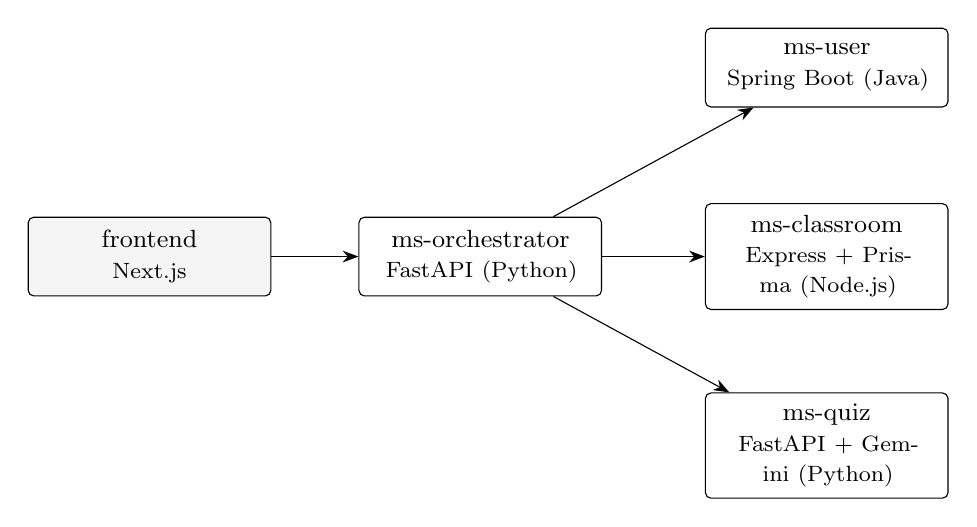
\begin{tikzpicture}[font=\small,
      caja/.style={draw,rounded corners=2pt,align=center,inner sep=4pt,
                   minimum height=10mm,text width=28mm},
      cajaext/.style={caja,fill=lightgray},
      flecha/.style={-{Stealth[length=2mm]}}]
    \node[cajaext] (fe) at (0,0) {frontend\\\footnotesize Next.js};
    \node[caja] (orch) at (4.2,0) {ms-orchestrator\\\footnotesize FastAPI (Python)};
    \node[caja] (user) at (8.6,2.4) {ms-user\\\footnotesize Spring Boot (Java)};
    \node[caja] (class) at (8.6,0) {ms-classroom\\\footnotesize Express + Prisma (Node.js)};
    \node[caja] (quiz) at (8.6,-2.4) {ms-quiz\\\footnotesize FastAPI + Gemini (Python)};

    \draw[flecha] (fe) -- (orch);
    \draw[flecha] (orch) -- (user);
    \draw[flecha] (orch) -- (class);
    \draw[flecha] (orch) -- (quiz);
  \end{tikzpicture}
  \caption{Arquitectura de KIWI. El frontend consume exclusivamente al orquestador, que a su vez
  distribuye cada petición al microservicio responsable del dominio.}
  \label{fig:arquitectura}
\end{figure}

\begin{table}[H]
\centering
\begin{tabular}{p{3.4cm}p{4cm}p{6cm}}
\toprule
\textbf{Componente} & \textbf{Tecnología} & \textbf{Responsabilidad}\\
\midrule
frontend & Next.js / TypeScript & Interfaz web para docentes y estudiantes.\\
ms-orchestrator & FastAPI / Python & API Gateway; enruta y compone llamadas.\\
ms-user & Spring Boot / Java & Autenticación y gestión de usuarios.\\
ms-classroom & Express + Prisma / Node.js & Aulas, estudiantes y competencias.\\
ms-quiz & FastAPI + Gemini / Python & Generación y gestión de quizzes.\\
PostgreSQL & PostgreSQL 13 & Persistencia compartida por esquemas/lógica de dominio.\\
\bottomrule
\end{tabular}
\caption{Componentes principales de KIWI.}
\end{table}

\section{Control de versiones con Git y Conventional Commits}
\label{sec:git}

\subsection{Qué son los Conventional Commits y por qué se usan}

Conventional Commits es una convención para escribir mensajes de commit con una estructura fija:
\texttt{tipo(alcance): descripción}, donde el tipo clasifica la naturaleza del cambio y el alcance,
opcional, indica qué parte del sistema afecta. El equipo la adoptó por tres razones concretas.
Primero, con cinco componentes independientes (frontend y cuatro servicios de backend), el alcance
del commit dice de inmediato en qué parte del sistema hay que mirar sin necesidad de abrir el
diff. Segundo, separa con claridad el trabajo de construir una funcionalidad nueva (\texttt{feat})
del de corregir un defecto (\texttt{fix}) o del de tareas de infraestructura
(\texttt{chore}), lo que vuelve legible el historial incluso para alguien que no participó en el
desarrollo. Tercero, es el estándar sobre el que se apoyan herramientas de generación automática de
\textit{changelogs} y de versionado semántico, algo relevante para un sistema que va a seguir
integrando componentes en la segunda mitad del curso.

\subsection{Tipos principales}

\begin{table}[htbp]
  \centering
  \caption{Tipos de Conventional Commits empleados en el historial del proyecto.}
  \label{tab:tipos-commit}
  \begin{tabularx}{\textwidth}{lX}
    \toprule
    \textbf{Tipo} & \textbf{Uso y ejemplo del historial} \\
    \midrule
    \texttt{feat}
      & Funcionalidad nueva y completa, casi siempre un microservicio entero al
        incorporarse por primera vez.\newline
        \emph{Ejemplo:} \texttt{feat(ms-quiz): add quiz management features} \\
    \addlinespace
    \texttt{fix}
      & Corrección de un defecto sobre código ya existente, sin agregar
        funcionalidad nueva.\newline
        \emph{Ejemplo:} \texttt{fix: stabilize service containers and return
        created quizzes} \\
    \addlinespace
    \texttt{docs}
      & Cambios que afectan únicamente a la documentación (README, guías,
        comentarios de API), sin tocar el código de ejecución.\newline
        \emph{Ejemplo:} \texttt{docs(readme): describe local setup with
        docker compose} \\
    \addlinespace
    \texttt{test}
      & Incorporación o modificación de pruebas unitarias, de integración o de
        extremo a extremo, sin alterar el comportamiento del sistema.\newline
        \emph{Ejemplo:} \texttt{test(ms-quiz): add unit tests for quiz
        service} \\
    \addlinespace
    \texttt{chore}
      & Tareas de mantenimiento o infraestructura que no cambian el
        comportamiento de negocio (setup de contenedores, configuración,
        dependencias).\newline
        \emph{Ejemplo:} \texttt{chore(ms-orchestrator): add container setup} \\
    \addlinespace
    \texttt{ci}
      & Cambios en la configuración o los scripts de integración y entrega
        continua (pipelines, workflows, automatización de despliegue).\newline
        \emph{Ejemplo:} \texttt{ci: add GitHub Actions workflow to build and
        test services} \\
    \addlinespace
    \texttt{refactor}
      & Reestructuración interna del código para mejorar su legibilidad o
        mantenibilidad, sin corregir defectos ni añadir funcionalidad.\newline
        \emph{Ejemplo:} \texttt{refactor(ms-quiz): extract validation logic
        into separate module} \\
    \bottomrule
  \end{tabularx}
\end{table}
\subsection{Metodología de ramificación}

El equipo sigue \textbf{Trunk Based Development (TBD)}: existe una única rama tronco,
\texttt{main}, que se mantiene siempre en un estado integrable, y cada microservicio o
característica se desarrolla en una rama de corta duración creada directamente desde
\texttt{main} (\texttt{feat/microservice-user}, \texttt{feat/microservice-classroom},
\texttt{feat/microservice-quiz}, \texttt{feat/orchestrator}, \texttt{feat/frontend},
\texttt{chore/docker-compose}). Esa rama temporal vive solo mientras dura la funcionalidad, se
integra a \texttt{main} mediante un Pull Request y se elimina inmediatamente después del merge; no
hay ramas de larga duración como \texttt{develop} o \texttt{release}, ni una jerarquía de ramas
entre sí, a diferencia de GitFlow. Esto es justamente lo que muestra el historial de la
Sección~\ref{sec:historial}: cada Pull Request nace de \texttt{main} y vuelve a \texttt{main},
nunca de otra rama de feature.

\subsection{Historial de commits}
\label{sec:historial}

El repositorio cuenta con 26 commits en \texttt{main} al momento de este informe. El Código~\ref{lst:gitlog} reproduce el historial completo
obtenido con \texttt{git log --oneline}.

\begin{lstlisting}[language=bash,caption={Historial de commits en \texttt{main} (\texttt{git log --oneline}).},label={lst:gitlog}]
825474f Merge pull request #6 from JeanPiero369/chore/docker-compose
3a3222b fix: stabilize service containers and return created quizzes
2047719 Merge pull request #5 from JeanPiero369/feat/frontend
9efe0b5 feat(frontend): add web application and core features
08466b1 Merge pull request #4 from JeanPiero369/feat/orchestrator
9b4fffe chore(ms-orchestrator): add container setup
7327962 feat(ms-orchestrator): add orchestration service
cdcbabd Merge pull request #3 from JeanPiero369/feat/microservice-quiz
1f0275b feat(ms-quiz): add quiz management features
5307ba5 Merge pull request #2 from JeanPiero369/feat/microservice-classroom
8115984 feat(ms-classroom): add classroom and student management
5d9fdc9 Merge pull request #1 from JeanPiero369/feat/microservice-user
f279c23 feat(ms-user): add authentication and user management
ef1aeca Initial commit
\end{lstlisting}

\begin{figure}[htbp]
  \centering
  \IfFileExists{images/commits.png}{%
    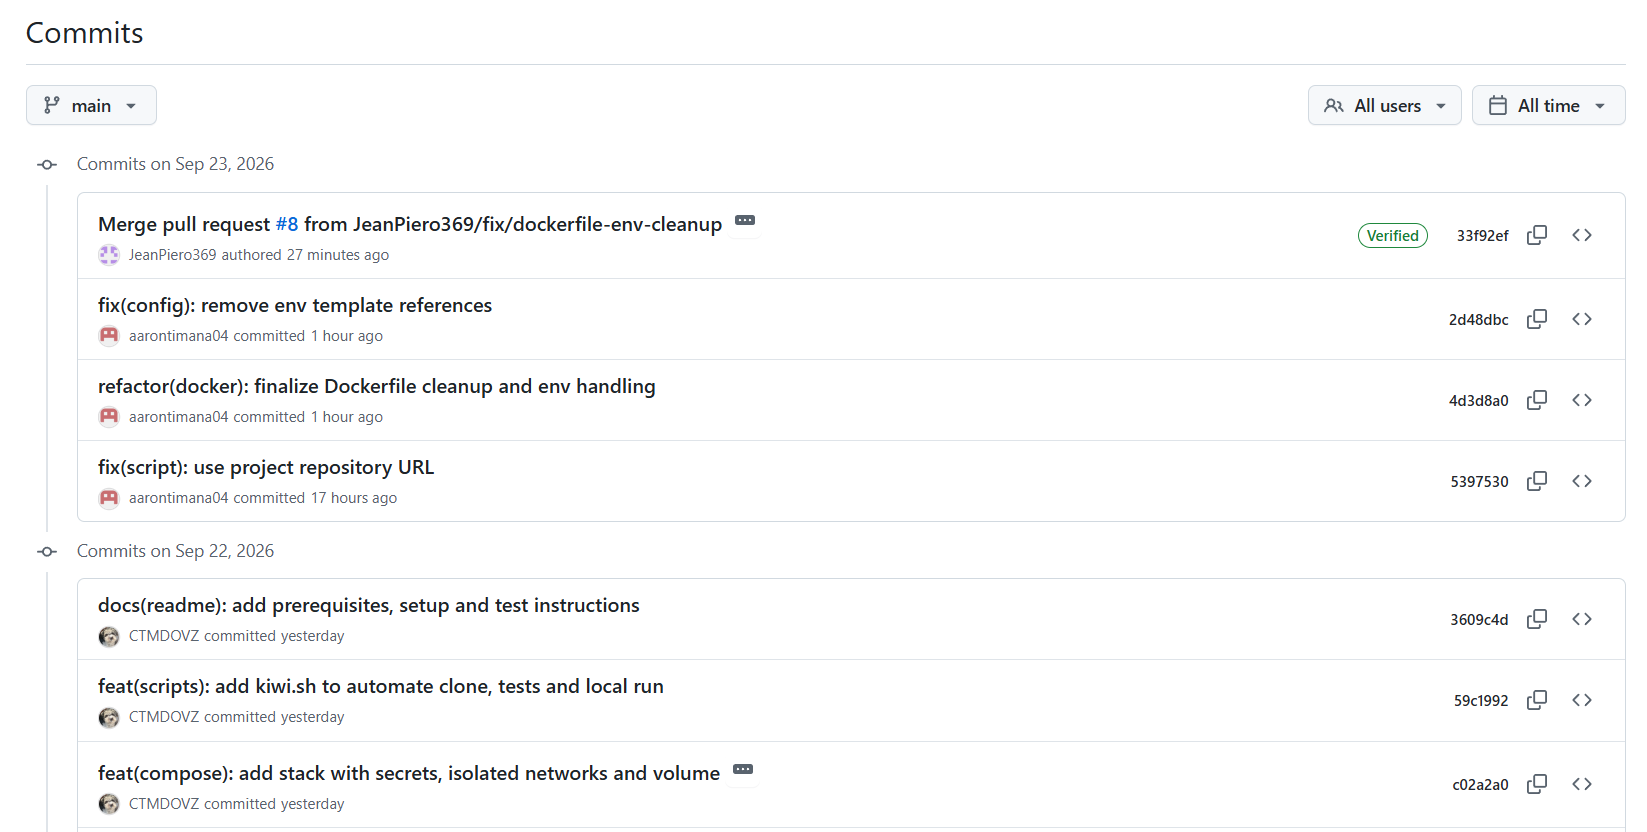
\includegraphics[width=\textwidth]{images/commits.png}}{}
  \caption{Historial de Commits.}
  \label{fig:commits}
\end{figure}

\subsection{Análisis detallado de una muestra de commits}
\label{sec:analisis-commits}

De los 26 commits del historial se seleccionaron 6 para un análisis más detallado, priorizando los
que corresponden a la incorporación de cada microservicio, que son los que más información aportan
sobre cómo creció el sistema.

\begin{description}[leftmargin=0pt,style=nextline,itemsep=8pt]

  \item[\texttt{f279c23} --- \texttt{feat(ms-user): add authentication and user management}]
  Primer microservicio incorporado al repositorio: 63 archivos y 2{,}125 líneas añadidas. Crea el
  proyecto Spring Boot completo (\texttt{pom.xml}, estructura Maven), su \texttt{Dockerfile}
  multi-etapa y la colección de peticiones de prueba manual (\texttt{api-endpoints/}) organizada
  en \texttt{Auth}, \texttt{Student} y \texttt{Teacher}. Establece el patrón que seguirán los
  demás microservicios: cada uno se agrega en un commit \texttt{feat} único que deja el servicio
  funcional y contenerizable desde el primer momento.

  \item[\texttt{8115984} --- \texttt{feat(ms-classroom): add classroom and student management}]
  Segundo microservicio, en Node.js con Express y Prisma: 43 archivos y 2{,}756 líneas. Introduce
  el esquema de base de datos (\texttt{prisma/schema.prisma}), las rutas de creación y consulta de
  aulas y la asociación de estudiantes, docentes y competencias a una clase. Es el servicio que
  mantiene la relación entre usuarios y quizzes asignados, y por eso es el que más endpoints de
  asociación expone (agregar estudiante, agregar docente, asociar competencia, asociar quiz).

  \item[\texttt{1f0275b} --- \texttt{feat(ms-quiz): add quiz management features}]
  Es el commit individual más grande del historial: 32 archivos y 4{,}901 líneas. Implementa la
  generación de quizzes con el modelo Gemini~2.0 Flash a partir de texto o de un PDF cargado por el
  usuario, la gestión de preguntas y respuestas, y el registro de intentos de un estudiante. Su
  tamaño refleja que es el microservicio con más lógica de negocio propia (procesamiento de PDF,
  llamadas al modelo de IA, cálculo de puntaje), a diferencia de los otros dos, que son
  mayormente CRUD.

  \item[\texttt{7327962} --- \texttt{feat(ms-orchestrator): add orchestration service}]
  Agrega la puerta de entrada en FastAPI: 51 archivos y 2{,}183 líneas, con un controlador por
  dominio (\texttt{\seqsplit{auth\_controller}}, \texttt{\seqsplit{student\_controller}},
  \texttt{\seqsplit{teacher\_controller}}, \texttt{\seqsplit{classroom\_controller}},
  \texttt{\seqsplit{quiz\_controller}}) que reenvía las peticiones del
  frontend a \texttt{ms-user}, \texttt{ms-classroom} y \texttt{ms-quiz} usando \texttt{httpx}.
  Este commit es el punto en el que el sistema deja de ser tres servicios sueltos y pasa a tener
  una única API coherente hacia afuera.

  \item[\texttt{9efe0b5} --- \texttt{feat(frontend): add web application and core features}]
  El commit más grande de todo el historial: 95 archivos y 22{,}844 líneas (la mayor parte,
  \texttt{package-lock.json}). Agrega la aplicación Next.js completa: el panel del docente
  (\texttt{dashboard/classrooms}, \texttt{dashboard/competencies}), el layout general y el cliente
  HTTP que consume al orquestador. Con este commit el sistema queda usable de punta a punta por
  primera vez, ya que hasta entonces los cuatro servicios de backend solo se podían probar con las
  colecciones de Bruno.

  \item[\texttt{3a3222b} --- \texttt{fix: stabilize service containers and return created quizzes}]
  Único commit de tipo \texttt{fix} del historial, con 7 archivos y 29 inserciones frente a 18
  eliminaciones. Corrige dos problemas distintos. El primero es de contenerización: los
  \texttt{Dockerfile} de \texttt{ms-quiz}, \texttt{ms-classroom}, \texttt{ms-orchestrator} y
  \texttt{ms-user} copiaban varios directorios de código fuente en una sola instrucción
  \texttt{COPY}, y se separó cada uno en su propia instrucción para evitar errores de build; de
  paso se reemplazó la imagen base \texttt{python:3.11-slim-buster}, ya sin soporte, por
  \texttt{python:3.11-slim}. El segundo es un defecto funcional real: el endpoint
  \texttt{createQuiz} de \texttt{ms-orchestrator} armaba la respuesta del microservicio de quizzes
  pero nunca la retornaba (\texttt{response.json()} se llamaba sin \texttt{return}), así que el
  frontend recibía un cuerpo vacío tras crear un quiz; y en el cliente HTTP del frontend, la
  llamada \texttt{createQuiz} envolvía la petición en un \texttt{try/catch} que absorbía cualquier
  error en silencio. Este commit es el ejemplo más claro del historial de por qué separar
  \texttt{fix} de \texttt{feat} importa: es un cambio pequeño y localizado, fácil de revisar en un
  Pull Request, que no habría sido visible si estuviera mezclado dentro de un commit de
  funcionalidad.

\end{description}

\subsection{Pull Requests}

Cada rama de funcionalidad se integró a \texttt{main} mediante un Pull Request, siguiendo la
metodología de ramificación descrita antes. La Tabla~\ref{tab:prs} resume los seis Pull Requests
del repositorio.

\begin{table}[htbp]
  \centering
  \caption{Pull Requests del repositorio y rama de origen.}
  \label{tab:prs}
  \begin{tabularx}{\textwidth}{clX}
    \toprule
    \textbf{PR} & \textbf{Rama} & \textbf{Contenido} \\
    \midrule
    \#1 & \texttt{feat/microservice-user}        & Autenticación y gestión de usuarios (ms-user) \\
    \#2 & \texttt{feat/microservice-classroom}    & Gestión de aulas y estudiantes (ms-classroom) \\
    \#3 & \texttt{feat/microservice-quiz}         & Generación y gestión de quizzes (ms-quiz) \\
    \#4 & \texttt{feat/orchestrator}               & Servicio orquestador (ms-orchestrator) \\
    \#5 & \texttt{feat/frontend}                   & Aplicación web (frontend) \\
    \#6 & \texttt{chore/docker-compose}            & Estabilización de contenedores de cada
                                                       servicio \\
    \bottomrule
  \end{tabularx}
\end{table}

\begin{figure}[htbp]
  \centering
  \IfFileExists{images/pullrequest.png}{%
    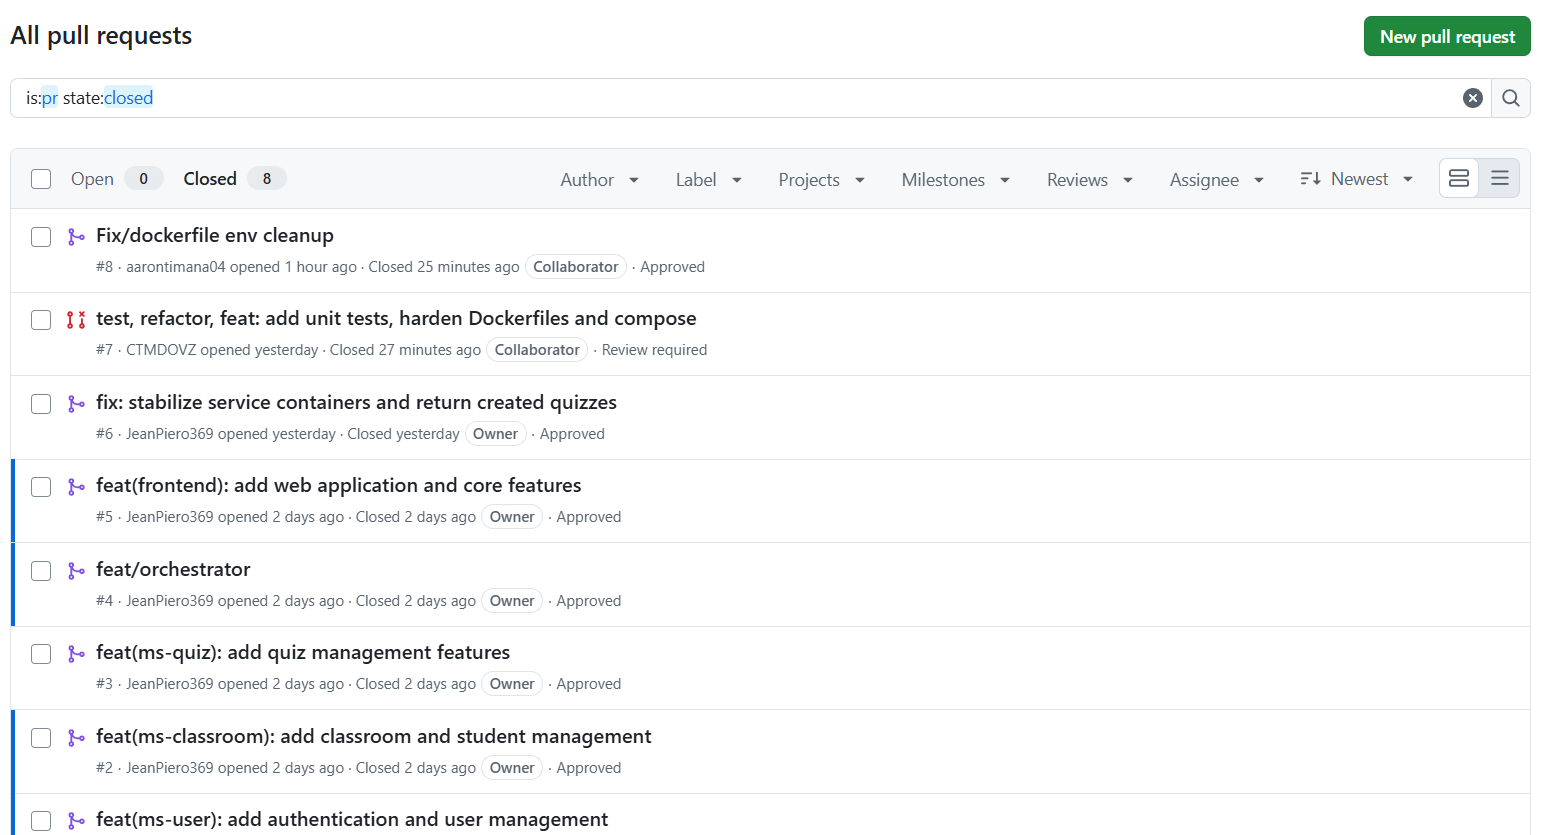
\includegraphics[width=\textwidth]{images/pullrequest.png}}{}
  \caption{Historial de pull request.}
  \label{fig:pullrequests}
\end{figure}


\section{Pruebas unitarias}
\subsection{Implementación actual}
La suite unitaria se concentra en \texttt{ms-orchestrator/tests/} y utiliza \textbf{pytest}. Para aislar el servicio de usuarios se usa \textbf{respx}, que intercepta las llamadas de \texttt{httpx}; por ello las pruebas no requieren levantar \texttt{ms-user} ni PostgreSQL.

Se implementaron \textbf{12 pruebas unitarias}: 7 validan DTOs de Pydantic y 5 ejercitan el controlador de autenticación.

\begin{itemize}[leftmargin=*]
\item Validación de login correcto, email inválido y límites de longitud del password.
\item Conversión y rechazo de roles inválidos.
\item Valores por defecto del modelo de estudiante.
\item Login exitoso con respuesta simulada del servicio de usuarios.
\item Propagación de error 401.
\item Respuesta 503 cuando el servicio de usuarios no está disponible.
\item Validación 422 que evita llamar al servicio externo con un body inválido.
\item Registro exitoso con respuesta simulada.
\end{itemize}

El comando documentado para ejecutarlas es:

\begin{lstlisting}
./kiwi.sh test
\end{lstlisting}

También pueden ejecutarse manualmente:

\begin{lstlisting}
cd ms-orchestrator
python3 -m venv .venv
source .venv/bin/activate
pip install -r requirements-dev.txt
pytest -v
\end{lstlisting}

\subsection{Evidencia de ejecución}
La ejecución local recolectó 12 casos y finalizó con \texttt{12 passed}. La advertencia visible corresponde a una deprecación de \texttt{starlette.testclient} y no representa una falla de las pruebas.

\begin{figure}[H]
\centering
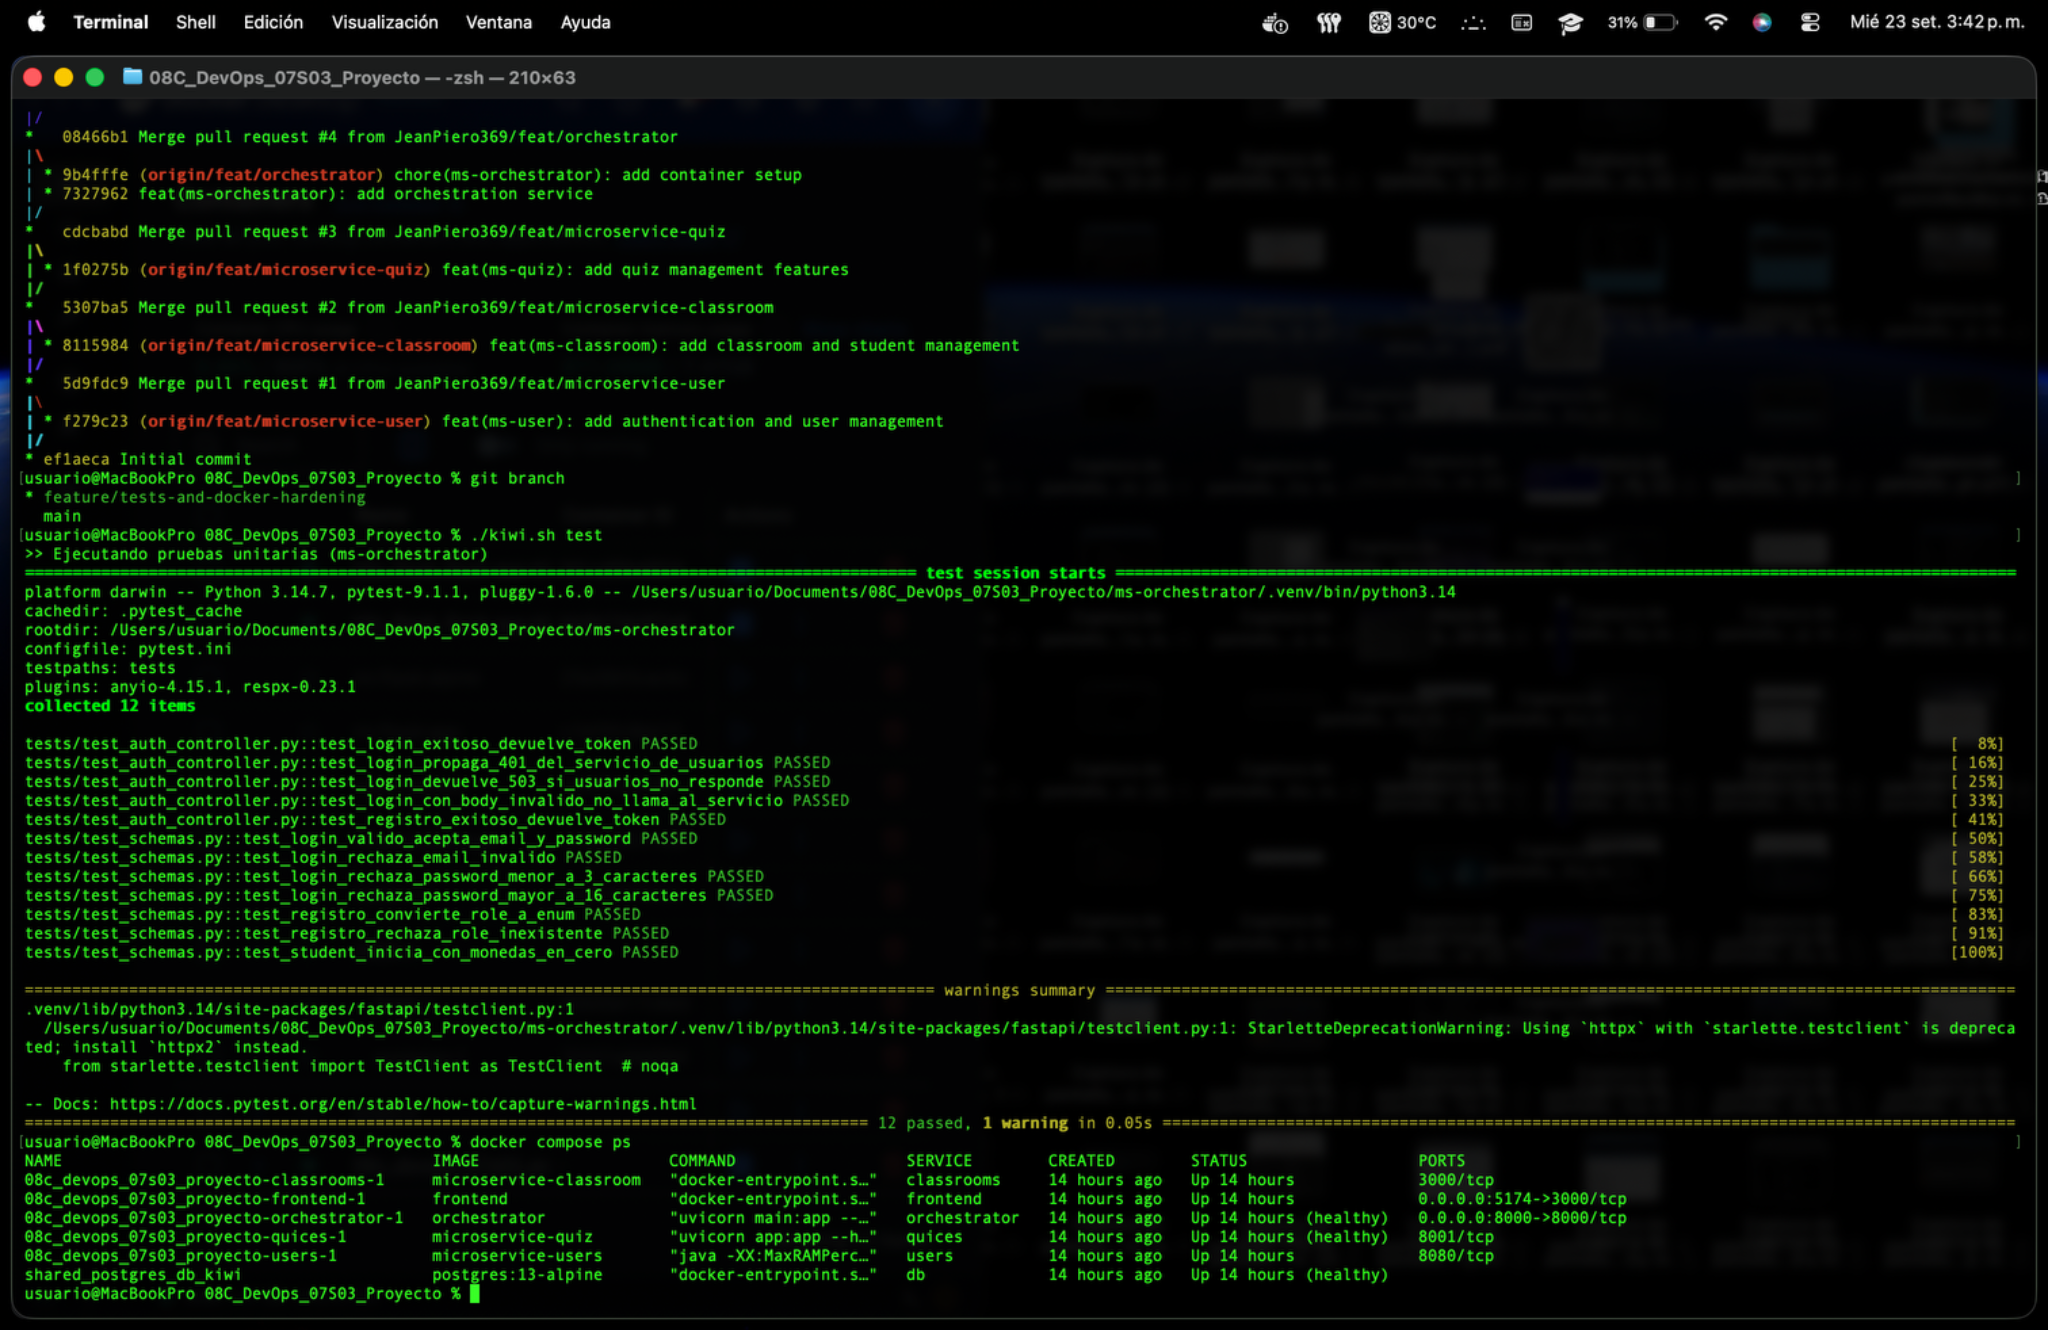
\includegraphics[width=0.98\textwidth]{images/tests_compose.png}
\caption{Ejecución de las 12 pruebas unitarias y estado de los contenedores mediante Docker Compose.}
\label{fig:testscompose}
\end{figure}

\section{Automatización con Bash}
El repositorio incorpora \texttt{kiwi.sh} en la raíz. El script unifica tareas repetitivas del entorno de desarrollo:

\begin{table}[H]
\centering
\begin{tabular}{p{4cm}p{9.5cm}}
\toprule
\textbf{Comando} & \textbf{Acción}\\
\midrule
\texttt{./kiwi.sh clone} & Clona o actualiza el repositorio.\\
\texttt{./kiwi.sh setup} & Verifica que exista \texttt{.env} y genera \texttt{secrets/db\_password.txt} a partir de \texttt{DB\_PASSWORD}.\\
\texttt{./kiwi.sh test} & Crea/reutiliza un entorno virtual e inicia pytest.\\
\texttt{./kiwi.sh up} & Ejecuta la preparación y construye/levanta el stack con Docker Compose.\\
\texttt{./kiwi.sh down} & Detiene el stack conservando el volumen.\\
\texttt{./kiwi.sh logs} & Muestra logs del stack o de un servicio.\\
\texttt{./kiwi.sh status} & Muestra el estado de los contenedores.\\
\bottomrule
\end{tabular}
\caption{Automatización disponible en \texttt{kiwi.sh}.}
\end{table}


\section{Dockerización de la aplicación}
\subsection{Dockerfiles}
Los componentes cuentan con Dockerfile adaptado a su runtime. La iteración final utiliza usuarios no root cuando corresponde, ordena las capas para favorecer el uso de caché y aplica builds multi-etapa en los servicios donde aporta una reducción del runtime. Durante la validación se mantuvieron instrucciones \texttt{COPY} separadas cuando eran necesarias para conservar la estructura de paquetes esperada por Python.

\begin{table}[H]
\centering
\begin{tabular}{p{3.5cm}p{6.5cm}p{2cm}}
\toprule
\textbf{Servicio} & \textbf{Base principal} & \textbf{Puerto}\\
\midrule
frontend & Node.js / Next.js multi-etapa & 3000\\
ms-user & Maven builder + Eclipse Temurin JRE & 8080\\
ms-classroom & node:18-alpine & 3000\\
ms-quiz & python:3.11-slim & 8001\\
ms-orchestrator & python:3.11-slim & 8000\\
\bottomrule
\end{tabular}
\caption{Resumen de contenerización.}
\end{table}

\subsection{Docker Compose}
El archivo \texttt{compose.yml} define el stack completo. PostgreSQL utiliza un volumen nombrado para persistencia y un healthcheck con \texttt{pg\_isready}. Los servicios de dominio esperan a que la base de datos esté saludable mediante \texttt{depends\_on} con \texttt{condition: service\_healthy}.

La topología de redes es deliberada:
\begin{itemize}[leftmargin=*]
\item \texttt{web}: conecta frontend con el orquestador.
\item \texttt{backend}: conecta el orquestador con los microservicios internos.
\item \texttt{data}: conecta microservicios con PostgreSQL y se declara \texttt{internal: true}.
\end{itemize}

Solo frontend y orquestador publican puertos al host. PostgreSQL no utiliza \texttt{ports}. La contraseña de la base se monta mediante un secret y el volumen \texttt{shared\_db\_data} conserva la información al ejecutar \texttt{docker compose down} sin \texttt{-v}.

\subsection{Evidencia de ejecución}
La evidencia de terminal de la Figura~\ref{fig:testscompose} muestra el stack levantado con \texttt{docker compose ps}; en esa validación los servicios se encontraban activos y los componentes con healthcheck reportaban estado saludable. Adicionalmente, se validó la exposición del orquestador mediante Swagger y el acceso al frontend de KIWI desde el navegador.

\begin{figure}[H]
\centering
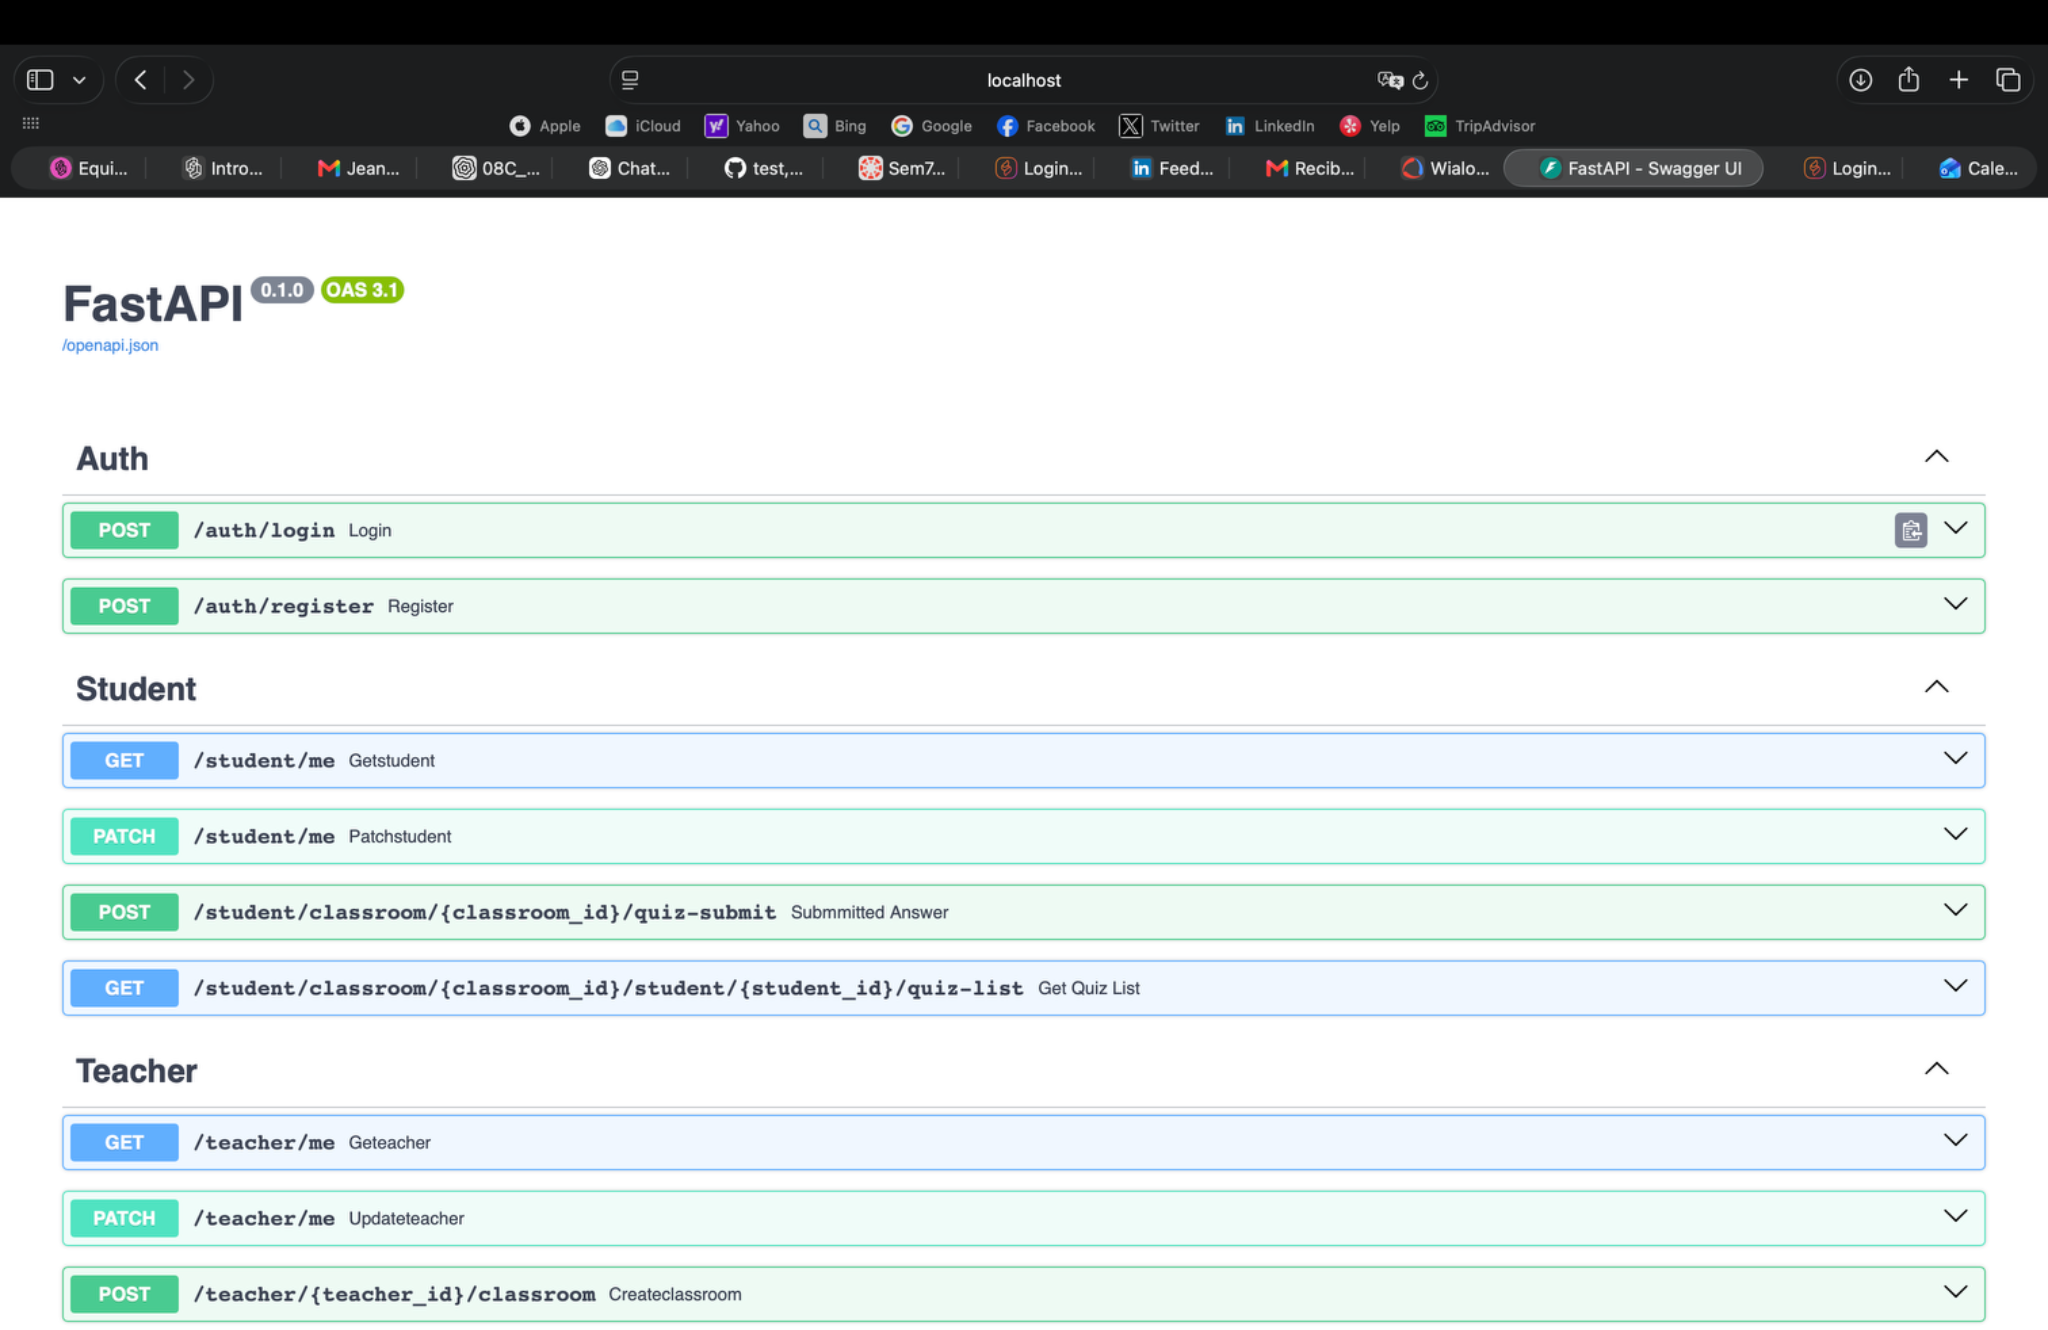
\includegraphics[width=0.98\textwidth]{images/swagger.png}
\caption{Swagger UI del orquestador disponible en \texttt{localhost:8000/docs}.}
\label{fig:swagger}
\end{figure}

\begin{figure}[H]
\centering
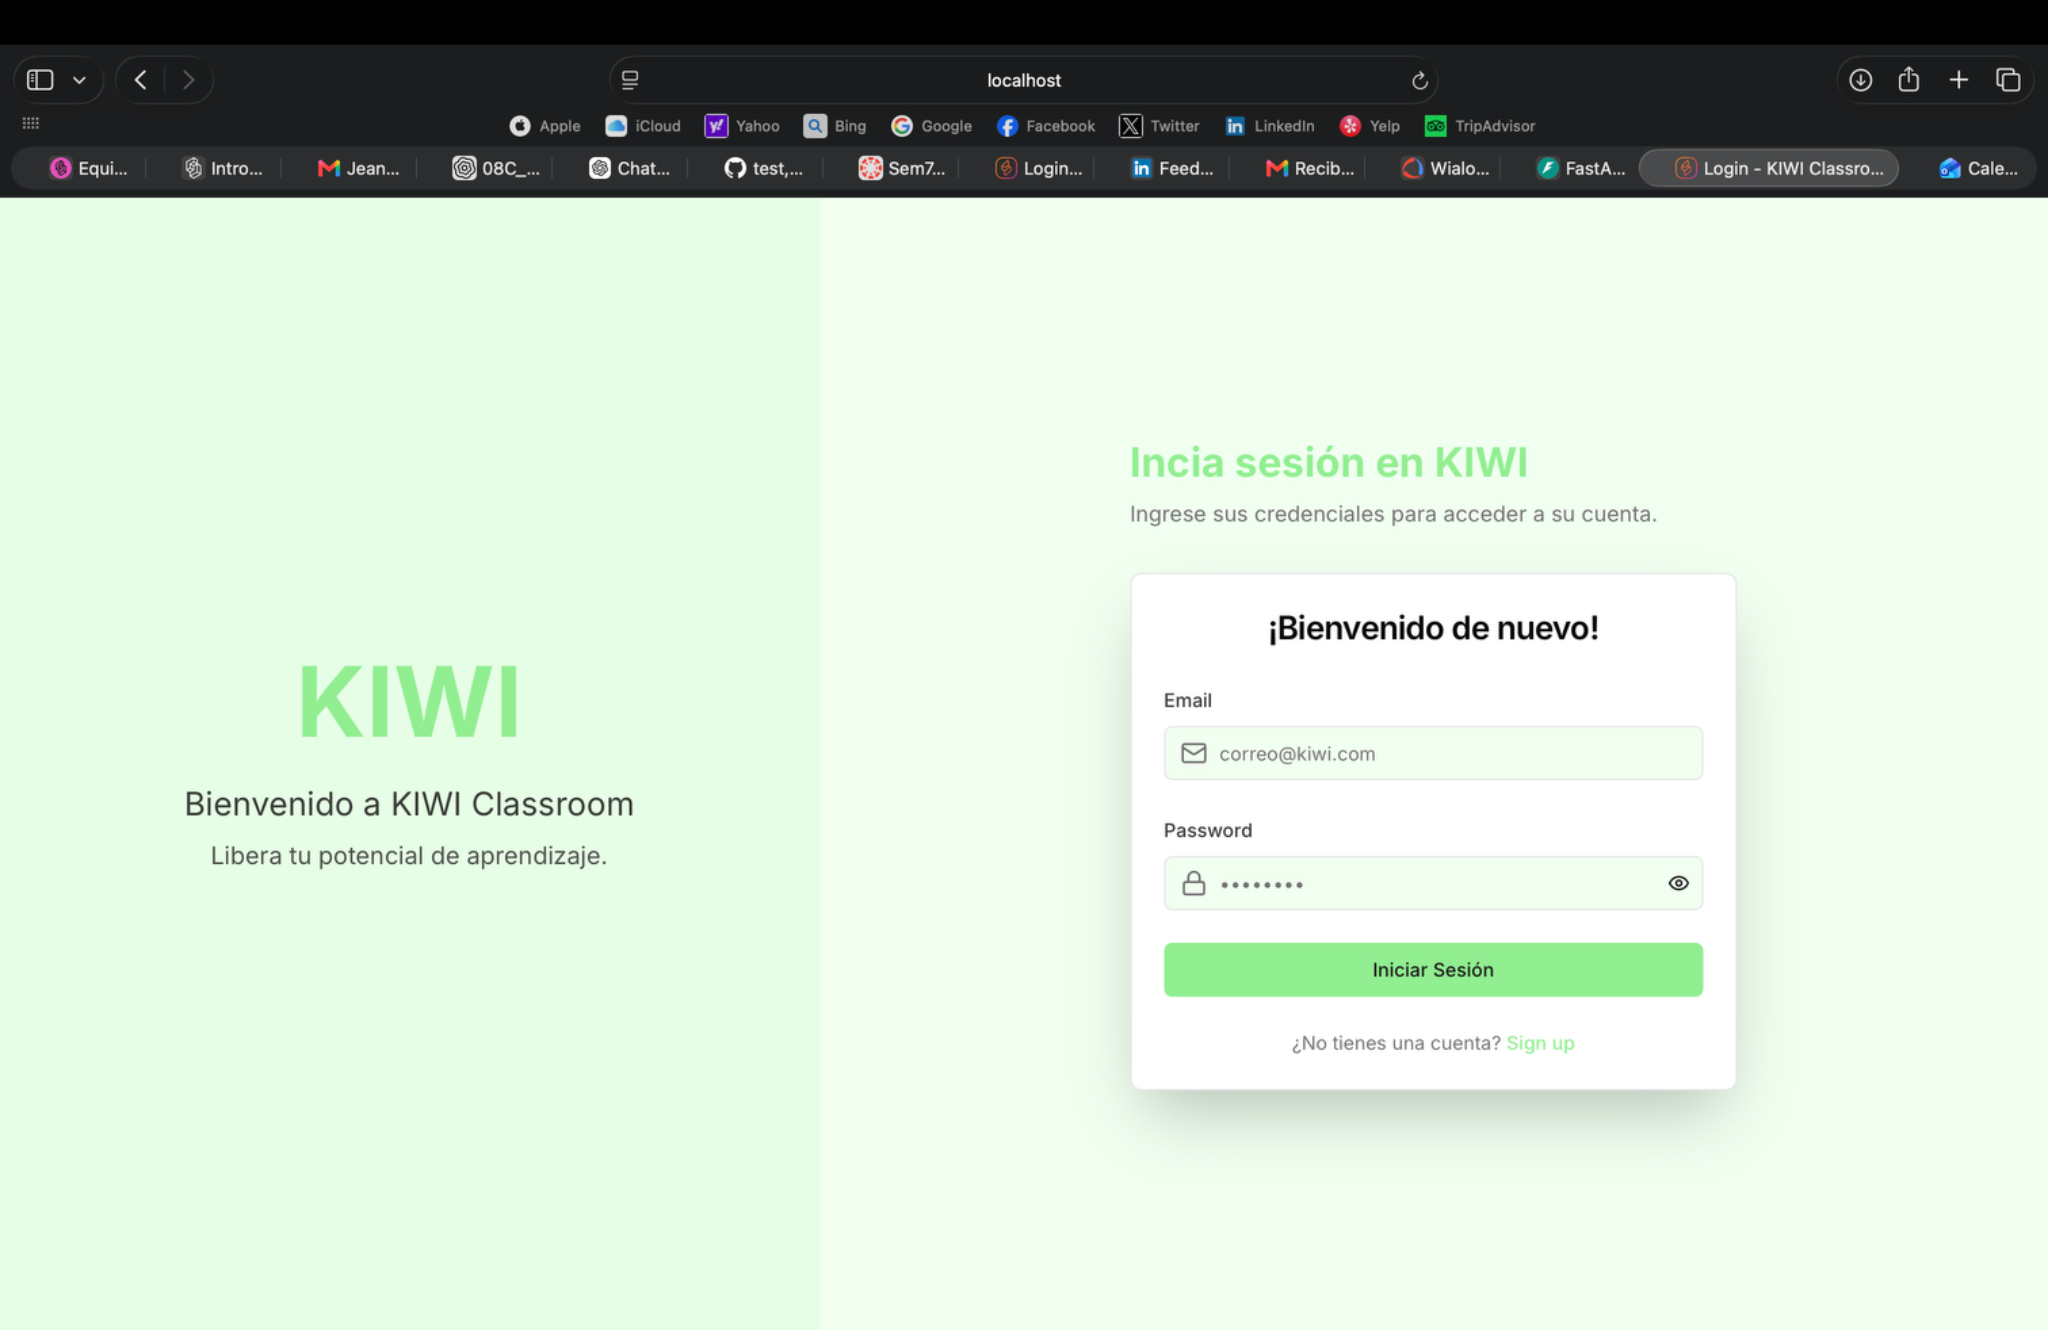
\includegraphics[width=0.98\textwidth]{images/frontend.png}
\caption{Frontend de KIWI disponible en \texttt{localhost:5174/login}.}
\label{fig:frontend}
\end{figure}

\section{Conclusiones del informe parcial}

El uso de Conventional Commits y Pull Requests permite reconstruir el crecimiento del sistema y distinguir funcionalidades, correcciones, infraestructura, pruebas y documentación. La estrategia de ramas cortas mantiene a \texttt{main} como punto de integración y resulta coherente con Trunk Based Development.

Se implementaron 12 pruebas unitarias aisladas, un script Bash para automatizar operaciones repetitivas y un \texttt{compose.yml} que orquesta frontend, orquestador, microservicios y PostgreSQL con redes, persistencia, healthcheck y manejo de credenciales fuera del repositorio. Las pruebas unitarias finalizan satisfactoriamente y tanto el frontend como la documentación Swagger del orquestador fueron comprobados en ejecución local.

\clearpage
\section{Informe final: alcance y evolución del proyecto}
\label{sec:alcance}

Este informe amplía el informe parcial. Conserva la descripción del producto, la arquitectura, el
control de versiones, las pruebas, la automatización con Bash y la dockerización, y añade el
trabajo DevSecOps exigido para la entrega final: modelo de amenazas STRIDE, análisis automático de
seguridad, centralización de hallazgos, mitigaciones, pipeline completo, monitoreo, madurez y
lecciones aprendidas. La Tabla~\ref{tab:rubrica} indica dónde se responde cada requisito.

Las cifras provienen de reportes reales: los artefactos de GitHub Actions, la instancia propia de
DefectDojo y las evidencias de \texttt{docs/devsecops/cierre}. Cada número se acompaña del run o
del archivo de origen. No se acredita operación productiva: lo demostrado es desarrollo local,
staging efímero en CI y publicación de imágenes desde \texttt{main}.

\begin{table}[htbp]
  \centering
  \caption{Correspondencia entre los requisitos del informe final y las secciones del documento.}
  \label{tab:rubrica}
  \small
  \begin{tabularx}{\textwidth}{cYl}
    \toprule
    \textbf{Req.} & \textbf{Contenido solicitado} & \textbf{Sección} \\
    \midrule
    a & Título y descripción del proyecto & \ref{sec:titulo} \\
    b & Diagrama STRIDE de la arquitectura & \ref{sec:stride} \\
    c & Explicación de las vulnerabilidades principales & \ref{sec:vulnerabilidades} \\
    d & Herramientas SAST y DAST, evidencias y reportes & \ref{sec:sast-dast} \\
    e & Secret scanning y análisis de dependencias (SCA) & \ref{sec:sca} \\
    f & Centralización de vulnerabilidades en DefectDojo & \ref{sec:defectdojo} \\
    g & Tabla de mitigaciones priorizada por severidad & \ref{sec:mitigaciones} \\
    h & Situación inicial frente a resultados & \ref{sec:resultados} \\
    i & Pipeline completo: diagrama y configuración & \ref{sec:pipeline} y Anexo~\ref{sec:anexo-yaml} \\
    j & Despliegue multiambiente y monitoreo & \ref{sec:ambientes} \\
    k & Modelo de madurez & \ref{sec:madurez} \\
    l & Lecciones aprendidas & \ref{sec:lecciones} \\
    m & Recomendaciones & \ref{sec:recomendaciones} \\
    --- & Enlaces al repositorio, diagrama draw.io y Excel STRIDE & \ref{sec:enlaces} \\
    \bottomrule
  \end{tabularx}
\end{table}

\subsection{Arquitectura de despliegue}

Fuera del stack de contenedores intervienen tres servicios externos: GitHub, que aloja el código y
ejecuta el pipeline; Google Gemini, que genera las preguntas, y Gmail SMTP, que envía los correos a
los usuarios. En la arquitectura objetivo del equipo, el frontend se aloja en AWS Amplify y el
backend corre con Docker Compose en una instancia AWS EC2. La Sección~\ref{sec:stride} detalla estos
flujos con sus fronteras de confianza.

\subsection{Evolución del repositorio}

Al cierre del informe parcial, \texttt{main} contaba con 26 commits; después de integrar el trabajo
DevSecOps (Pull Requests \#11 a \#13) cuenta con 69, incluidos los de merge. La
Tabla~\ref{tab:prs-final} lista los Pull Requests posteriores al informe parcial, que siguen la misma
metodología de ramas cortas hacia \texttt{main}.

\begin{table}[htbp]
  \centering
  \caption{Pull Requests posteriores al informe parcial.}
  \label{tab:prs-final}
  \begin{tabularx}{\textwidth}{clX}
    \toprule
    \textbf{PR} & \textbf{Rama} & \textbf{Contenido} \\
    \midrule
    \#7 & \texttt{feature/tests-and-docker-hardening} & Pruebas y endurecimiento de Docker
                                                       (cerrado sin merge) \\
    \#8 & \texttt{fix/dockerfile-env-cleanup}       & Limpieza de Dockerfiles y variables de
                                                       entorno \\
    \#9 & \texttt{aarontimana04-patch-1}            & Carga de archivos desde la web de GitHub \\
    \#10 & \texttt{fix/compose}                    & URL del backend en Compose \\
    \#11 & \texttt{feat/devsecops-pipeline}        & Pipeline DevSecOps, modelo STRIDE y línea
                                                       base de seguridad \\
    \#12 & \texttt{fix/security-mitigations}       & Mitigación de amenazas STRIDE y hallazgos
                                                       de CI \\
    \#13 & \texttt{fix/project-closure}            & Gate de seguridad, parches de Spring y
                                                       cierre \\
    \bottomrule
  \end{tabularx}
\end{table}

\subsection{Ampliación de las pruebas}

Las mitigaciones de seguridad se acompañaron de pruebas que verifican cada control, incluidas
pruebas negativas: qué responde el sistema cuando un usuario intenta actuar sobre recursos ajenos
o registrarse con un rol que no le corresponde. El pipeline ejecuta las suites de Python y Java en
cada push (Sección~\ref{sec:pipeline}). La Tabla~\ref{tab:pruebas-cierre} resume la validación
registrada en \ruta{docs/devsecops/cierre/VALIDACION.md}.

\begin{table}[htbp]
  \centering
  \caption{Pruebas automatizadas y comprobaciones del cierre.}
  \label{tab:pruebas-cierre}
  \small
  \begin{tabularx}{\textwidth}{L{4.6cm}cY}
    \toprule
    \textbf{Suite} & \textbf{Correctas} & \textbf{Qué verifica} \\
    \midrule
    pytest del gateway & 31 & Esquemas, controlador de autenticación y autorización por la
    identidad del token (IDs ajenos, roles) \\
    pytest de ms-quiz & 6 & Límites de tamaño y páginas, archivos que no son PDF y PDF corruptos \\
    JUnit de seguridad (ms-user) & 10 & Rol asignado por el servidor, invitación docente y
    validación del encabezado del token \\
    Integración BootMigrationTest & 3 & Login, respuesta sin contraseña, token alterado, invitación
    docente y PATCH sin cambio de rol, monedas ni contraseña, con PostgreSQL aislado \\
    Validadores de reportes y URLs & 3 & Reportes que exige el gate y URLs permitidas para las
    sondas (\ruta{security/scripts}) \\
    \midrule
    \textbf{Total automatizado} & \textbf{53} & Sin fallos ni omisiones \\
    E2E local & 16 & Perfiles y controles de seguridad sobre el stack completo \\
    \bottomrule
  \end{tabularx}
\end{table}

\section{Modelo de amenazas STRIDE}
\label{sec:stride}

\subsection{Método}

El modelo se construyó en draw.io a partir de \ruta{compose.yml}, del \ruta{README.md} y del código
de los microservicios, siguiendo las tres preguntas del modelado de amenazas. La primera hoja del
archivo responde \emph{qué estamos construyendo} (Figura~\ref{fig:stride-arq}); la segunda,
\emph{qué puede salir mal}, con el diagrama de flujo de datos (DFD) y las amenazas STRIDE
(Figura~\ref{fig:stride-dfd}); la tercera, \emph{qué haremos al respecto}, con la plantilla de
evaluación del curso (Figura~\ref{fig:stride-plantilla}). El archivo draw.io con las tres hojas
está disponible en el enlace de la Sección~\ref{sec:enlaces}.

El DFD distingue actores (desarrollador, estudiante y docente), procesos (frontend, orchestrator,
ms-user, ms-classroom y ms-quiz), almacenes de datos (\texttt{localStorage} del navegador y
PostgreSQL) y entidades externas (GitHub, Gmail SMTP y Gemini). Separa siete fronteras de
confianza: GitHub, AWS Amplify, dispositivo del usuario, AWS EC2 con Docker Compose, red
\texttt{data} interna, Gmail y Gemini. Cada amenaza se marca sobre el elemento o flujo que afecta
con su letra STRIDE y un identificador T1--T17.

La Tabla~\ref{tab:stride-categorias} resume las seis categorías y la propiedad de seguridad que
cada una vulnera. Se identificaron 17 amenazas: cuatro de suplantación, cuatro de manipulación, dos
de repudio, cuatro de divulgación de información, una de denegación de servicio y dos de elevación
de privilegios. Seis de ellas, una por categoría, se priorizaron y evaluaron con la plantilla
(Sección~\ref{sec:vulnerabilidades}).

\begin{table}[htbp]
  \centering
  \caption{Categorías STRIDE y propiedad de seguridad afectada.}
  \label{tab:stride-categorias}
  \small
  \begin{tabularx}{\textwidth}{clY}
    \toprule
    \textbf{Letra} & \textbf{Amenaza} & \textbf{Propiedad afectada} \\
    \midrule
    S & Spoofing (suplantación de identidad) & Autenticación \\
    T & Tampering (manipulación de datos) & Integridad \\
    R & Repudiation (repudio) & No repudio \\
    I & Information Disclosure (divulgación de información) & Confidencialidad \\
    D & Denial of Service (denegación de servicio) & Disponibilidad \\
    E & Elevation of Privilege (escalamiento de privilegios) & Autorización \\
    \bottomrule
  \end{tabularx}
\end{table}

\begin{landscape}
\begin{figure}[p]
  \centering
  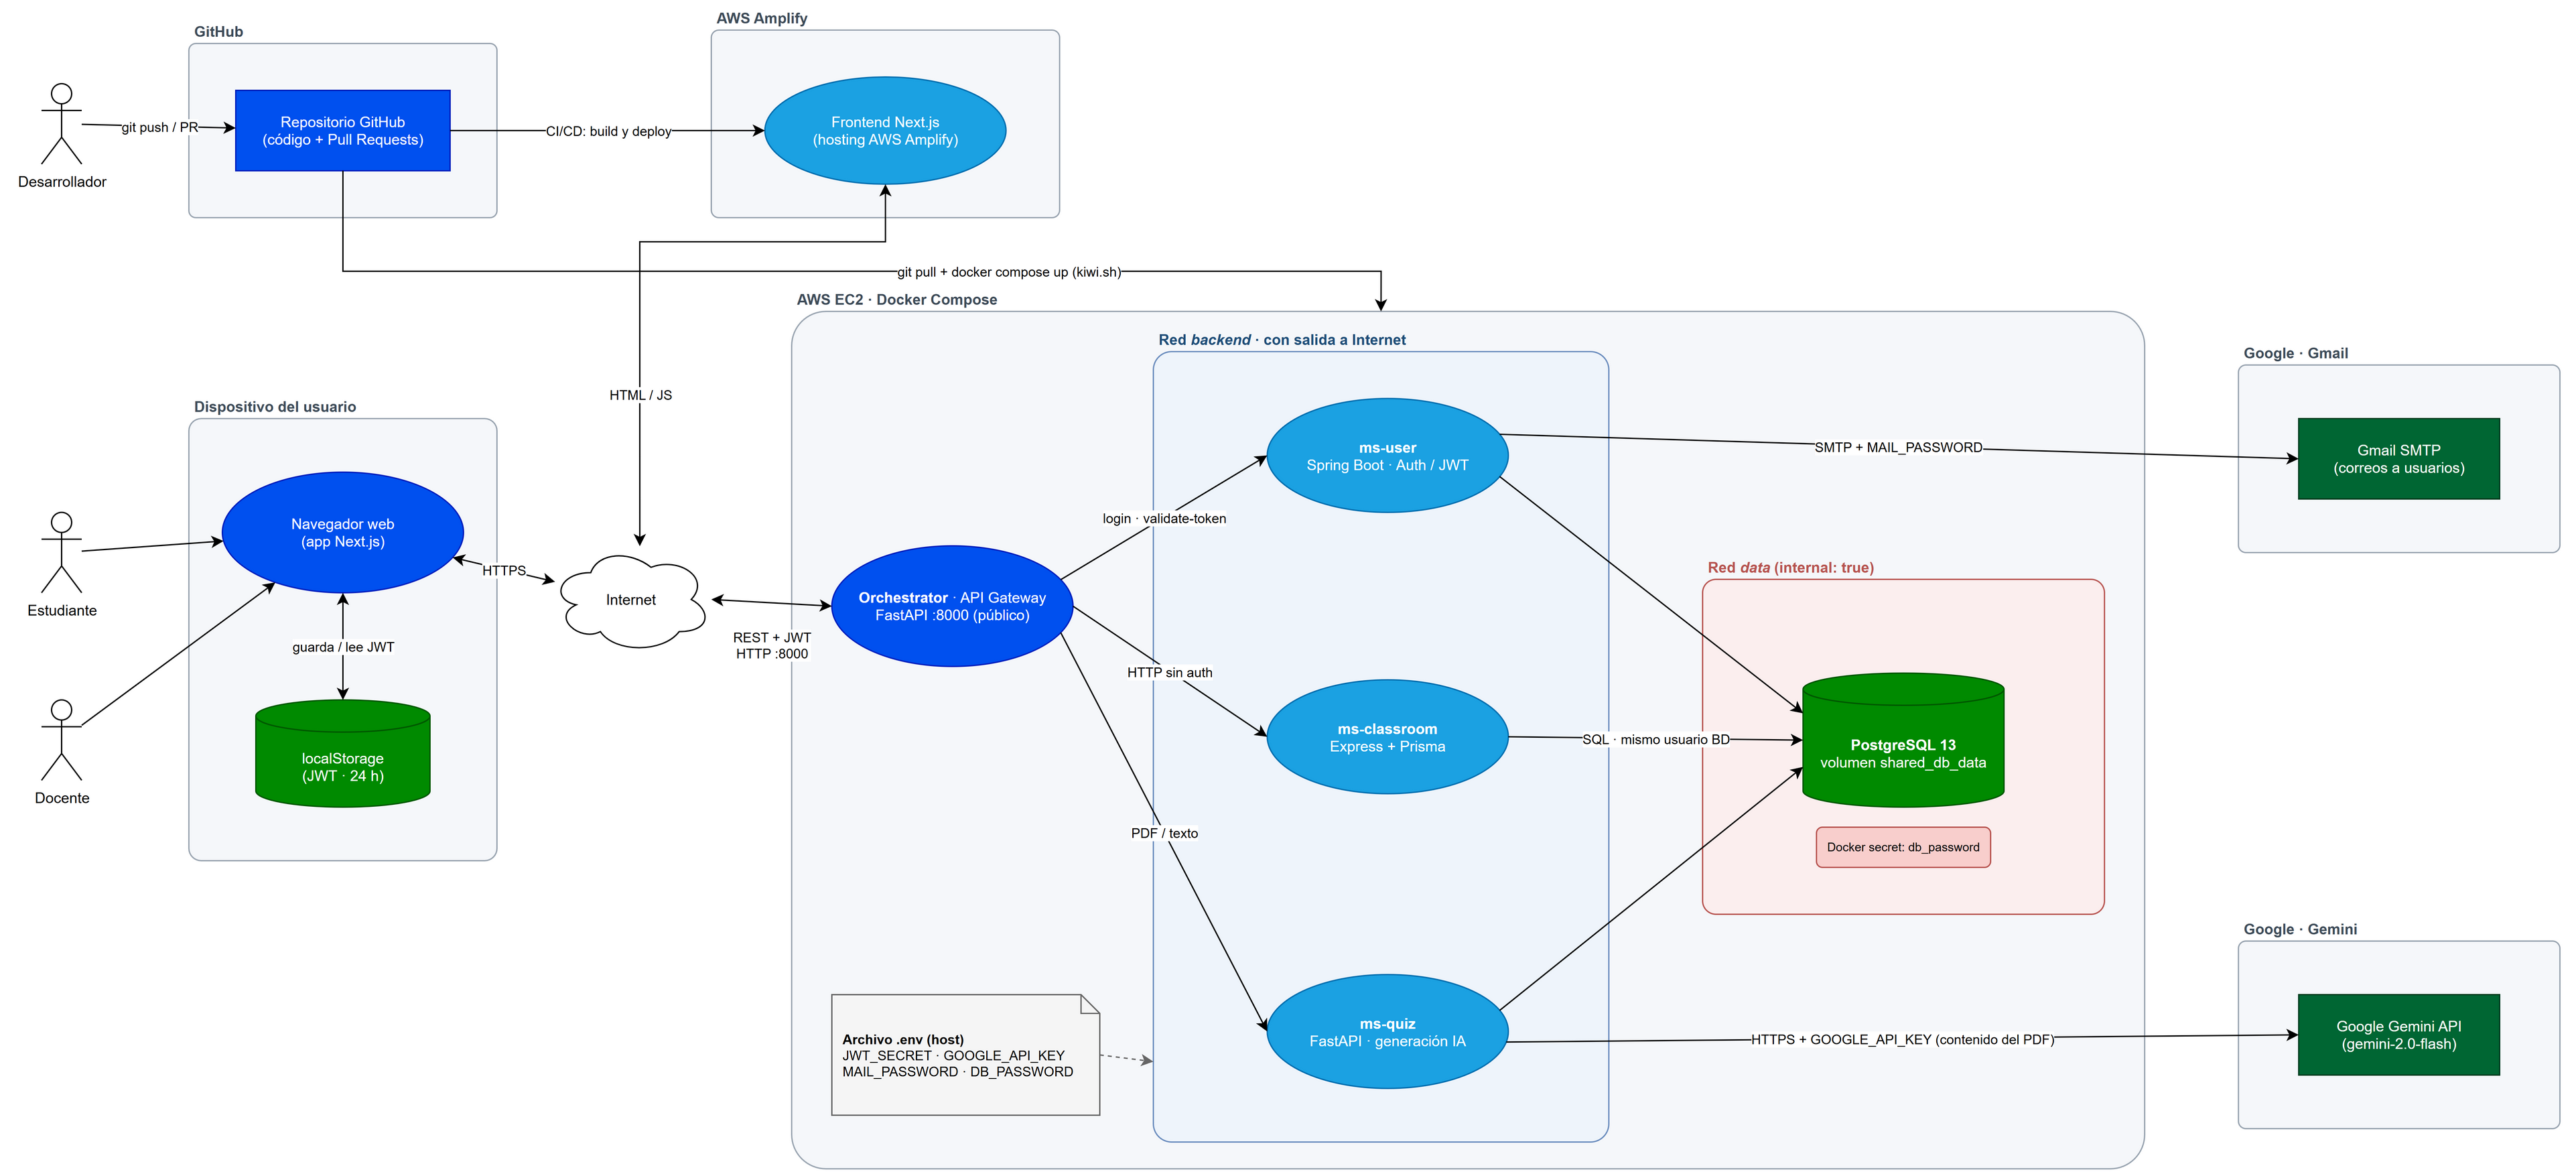
\includegraphics[width=\linewidth,height=0.82\textheight,keepaspectratio]{stride-arquitectura.png}
  \caption{Hoja 1 del modelo: arquitectura de KIWI con sus redes Docker (\texttt{backend} con
  salida a Internet y \texttt{data} interna), el archivo \texttt{.env} del host y los servicios
  externos. Fuente editable: \ruta{diagramas/STRIDE.drawio}.}
  \label{fig:stride-arq}
\end{figure}
\end{landscape}

\begin{landscape}
\begin{figure}[p]
  \centering
  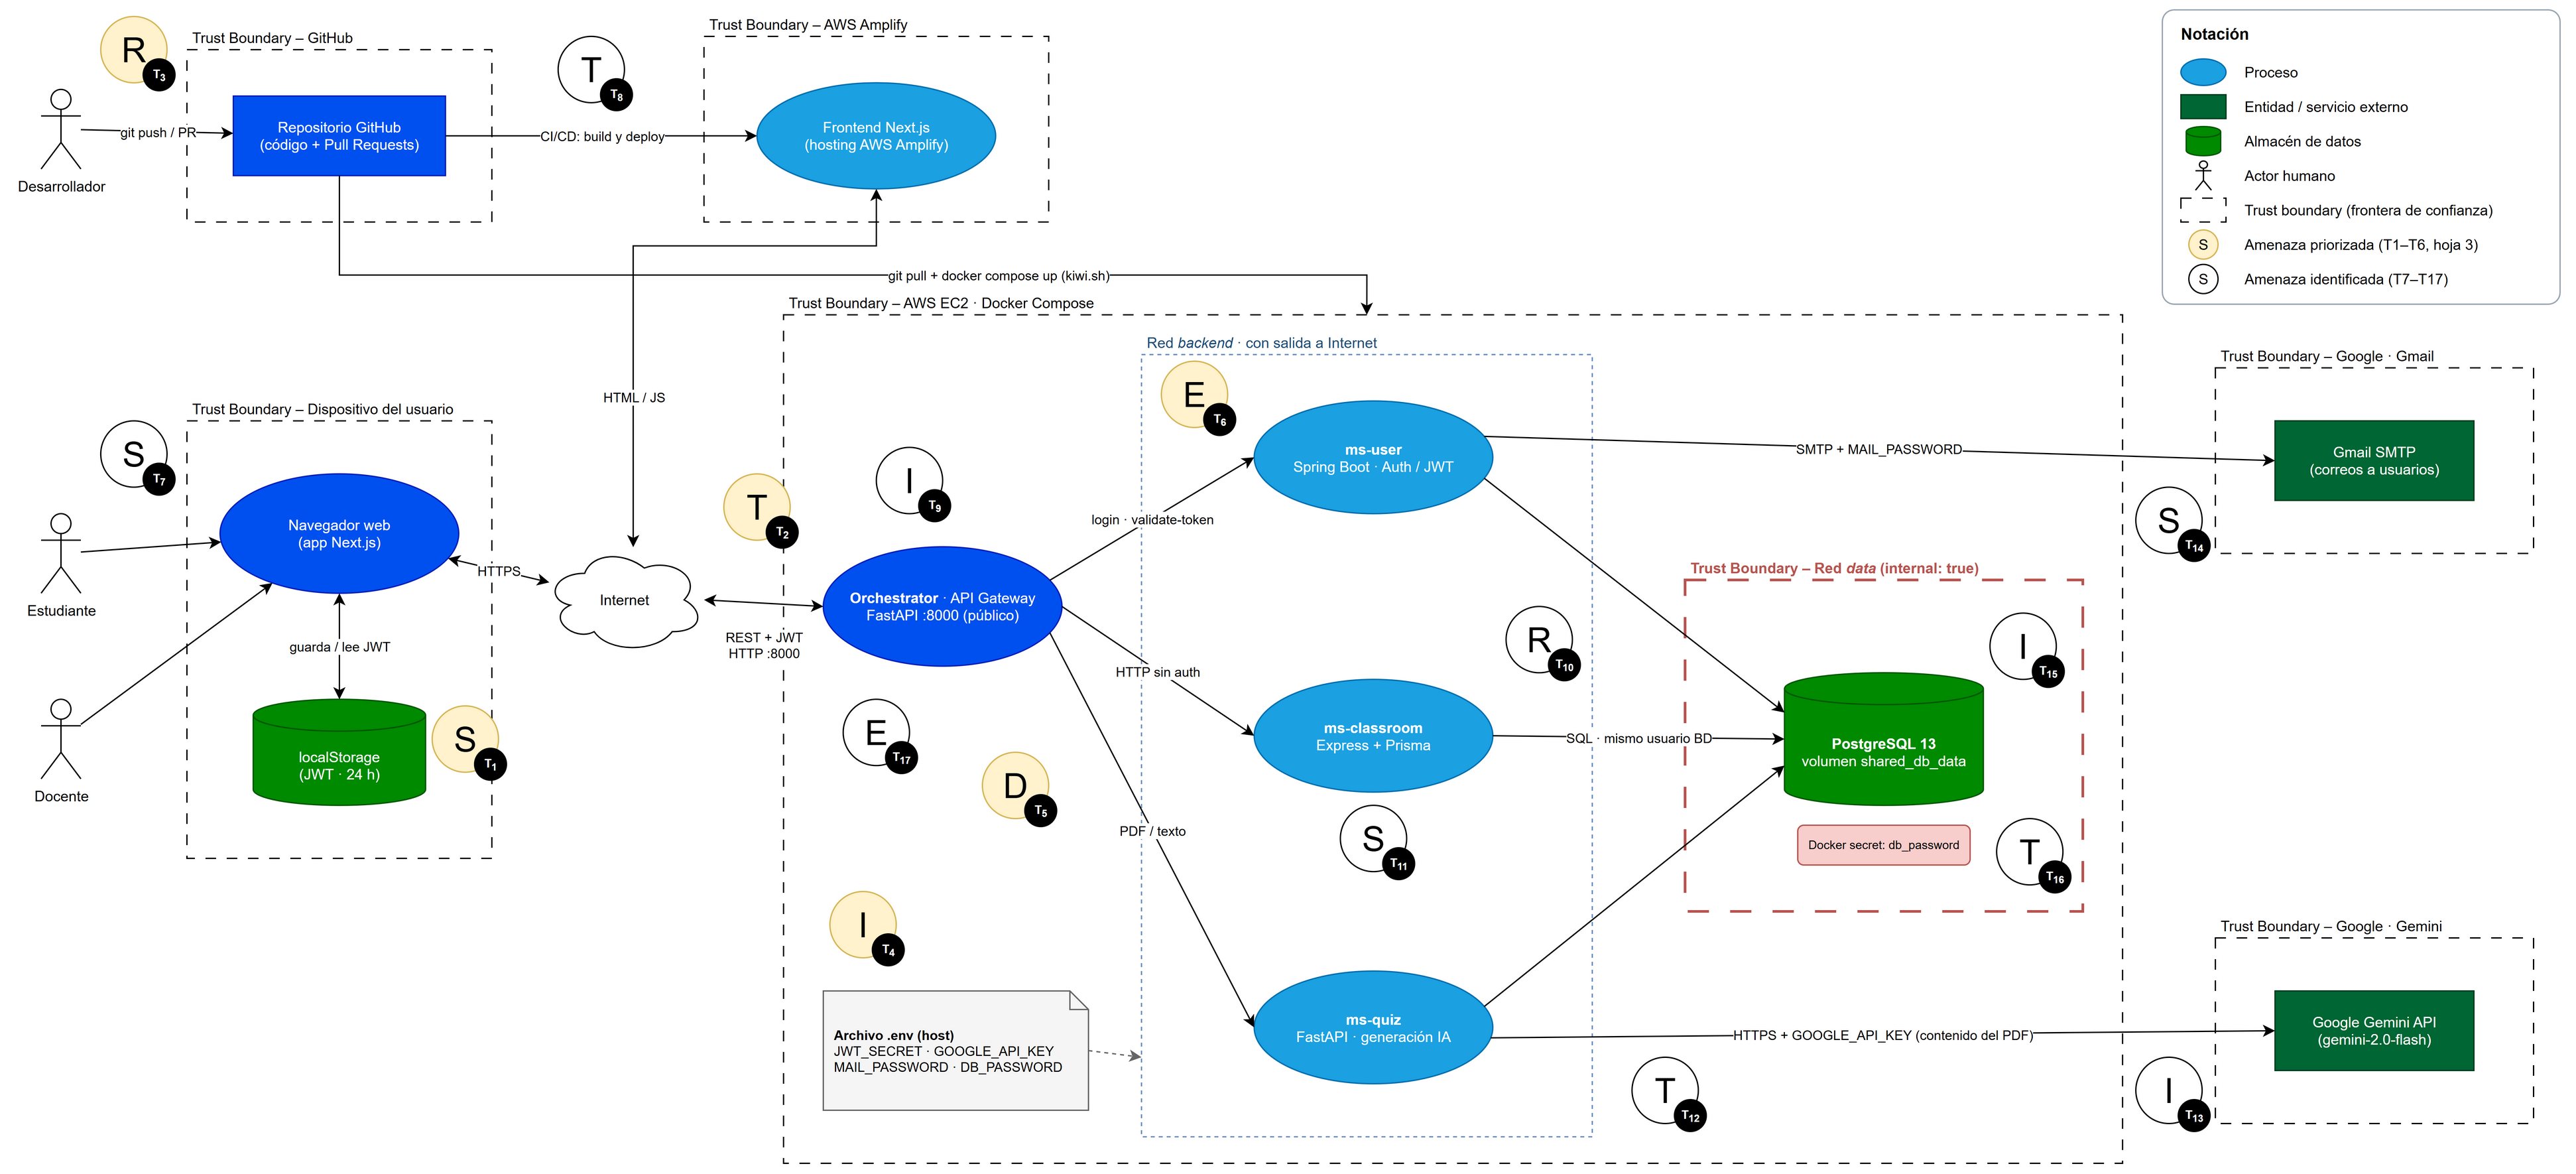
\includegraphics[width=\linewidth,height=0.82\textheight,keepaspectratio]{stride-amenazas.png}
  \caption{Hoja 2 del modelo: DFD con fronteras de confianza y las 17 amenazas STRIDE. En amarillo,
  las seis priorizadas (T1--T6); en blanco, las demás identificadas (T7--T17). El archivo
  draw.io muestra la descripción de cada marcador al pasar el cursor.}
  \label{fig:stride-dfd}
\end{figure}
\end{landscape}

\subsection{Catálogo de amenazas identificadas}

La Tabla~\ref{tab:catalogo} reproduce el catálogo de la hoja 2. Describe la situación modelada sobre
la línea base del proyecto; el estado de las amenazas priorizadas después de las mitigaciones se
analiza en la Sección~\ref{sec:vulnerabilidades}.

{\small
\begin{longtable}{L{0.8cm}L{0.6cm}L{3.3cm}L{9.6cm}}
  \caption{Catálogo de las 17 amenazas STRIDE del DFD de KIWI.}\label{tab:catalogo}\\
  \toprule
  \textbf{ID} & & \textbf{Componente o flujo} & \textbf{Amenaza} \\
  \midrule
  \endfirsthead
  \toprule
  \textbf{ID} & & \textbf{Componente o flujo} & \textbf{Amenaza} \\
  \midrule
  \endhead
  \bottomrule
  \endfoot
  T1 & S & Navegador, sesión JWT & Robo del JWT guardado en \texttt{localStorage} (por XSS o en
  un equipo compartido) para suplantar a un docente o estudiante; el token dura 24~h y no se
  puede revocar. \\
  T2 & T & Navegador y orchestrator & El orchestrator se publica por HTTP en el puerto 8000 sin
  terminación TLS; un atacante en la red puede alterar respuestas, notas o envíos de quiz. \\
  T3 & R & Desarrollador y GitHub & Los commits no están firmados y no hay revisión obligatoria
  verificable: un desarrollador puede introducir código malicioso y negar su autoría. \\
  T4 & I & Secretos del \texttt{.env} & \texttt{JWT\_SECRET}, \texttt{GOOGLE\_API\_KEY},
  \texttt{MAIL\_PASSWORD} y \texttt{DB\_PASSWORD} llegan como variables de entorno en texto plano;
  con \texttt{JWT\_SECRET} se pueden forjar tokens de cualquier usuario. \\
  T5 & D & Orchestrator y ms-quiz (PDF) & La generación desde PDF no limitaba tamaño ni frecuencia:
  el archivo se leía completo en memoria y cada petición consumía cuota de Gemini. \\
  T6 & E & ms-user, registro & El cliente elegía su rol al registrarse: cualquiera podía crear
  una cuenta TEACHER y acceder a aulas, quizzes y resultados. \\
  T7 & S & Estudiante y docente & Phishing o fuerza bruta de credenciales: el login no tiene MFA,
  bloqueo por intentos ni límite de frecuencia. \\
  T8 & T & Pipeline GitHub y Amplify & Una dependencia npm comprometida o un cambio no revisado
  alteran el bundle que Amplify publica a todos los usuarios. \\
  T9 & I & Orchestrator & Swagger público y CORS permisivo exponen la superficie completa de la
  API y permiten invocarla desde cualquier origen. \\
  T10 & R & Orchestrator y ms-classroom & No hay logs de auditoría con la identidad del usuario:
  un estudiante puede negar un envío o un docente un cambio de notas. \\
  T11 & S & ms-classroom & El servicio no autentica a quien lo llama: un contenedor comprometido
  de la red \texttt{backend} puede hacerse pasar por el orchestrator. \\
  T12 & T & ms-quiz y Gemini & Una inyección de instrucciones en el PDF o el texto manipula las
  preguntas o las respuestas correctas generadas. \\
  T13 & I & ms-quiz y Gemini & El contenido de los PDF, con posibles datos de alumnos, se envía
  a un tercero sin anonimizar. \\
  T14 & S & ms-user y Gmail SMTP & Los correos salen de una cuenta Gmail genérica, sin dominio
  propio con SPF, DKIM y DMARC, lo que facilita imitar a KIWI. \\
  T15 & I & PostgreSQL & Los tres microservicios comparten usuario de base de datos y el volumen
  no tiene cifrado configurado. \\
  T16 & T & PostgreSQL & Con el usuario compartido, un servicio comprometido puede modificar tablas
  de otros dominios (usuarios, notas, monedas). \\
  T17 & E & Orchestrator (IDOR) & Solo se validaba el rol del token, no que el
  \texttt{teacher\_id} o \texttt{userId} recibido fuera el del usuario autenticado; por ejemplo,
  comprar personajes con monedas ajenas. \\
\end{longtable}
}

\section{Vulnerabilidades principales}
\label{sec:vulnerabilidades}

Se priorizó una amenaza por categoría STRIDE, lo que cubre las cinco vulnerabilidades principales
que pide el informe y añade la sexta categoría. La Tabla~\ref{tab:top-stride} sigue el formato del
ejemplo del enunciado.

\begin{table}[htbp]
  \centering
  \caption{Amenazas priorizadas del modelo STRIDE.}
  \label{tab:top-stride}
  \small
  \begin{tabularx}{\textwidth}{L{2.6cm}L{3.4cm}Y}
    \toprule
    \textbf{Tipo de amenaza} & \textbf{Componente} & \textbf{Descripción} \\
    \midrule
    Spoofing (T1) & Sesión JWT en el navegador & Robo y reutilización del token guardado en
    \texttt{localStorage} para suplantar a un usuario. \\
    \addlinespace
    Tampering (T2) & Flujo navegador--orchestrator & Tráfico HTTP sin TLS hacia el puerto 8000,
    expuesto a manipulación en tránsito. \\
    \addlinespace
    Repudiation (T3) & Desarrollador y repositorio & Commits sin firma ni revisión obligatoria
    verificable; la autoría de un cambio puede negarse. \\
    \addlinespace
    Information Disclosure (T4) & Secretos del stack & Claves y contraseñas en variables de
    entorno y JWT versionados en el historial de Git. \\
    \addlinespace
    Denial of Service (T5) & Generación de quizzes desde PDF & Archivos grandes o ráfagas de
    peticiones agotan memoria y cuota de IA. \\
    \addlinespace
    Elevation of Privilege (T6) & Registro de ms-user & El cliente podía autoasignarse el rol
    docente. \\
    \bottomrule
  \end{tabularx}
\end{table}

\subsection{Evaluación del riesgo}

La evaluación usa la plantilla STRIDE del curso. El riesgo inherente se asigna con la hoja de
evaluación y su escala de riesgo; la efectividad del control vigente, con la escala de controles, y
de ambos resulta el riesgo residual. Con un apetito de riesgo de 3 - Moderate, una amenaza solo se
considera mitigada si su riesgo residual queda por debajo de ese nivel. La plantilla se evaluó sobre
la línea base; la columna \emph{Estado en el cierre} registra lo verificado en el código integrado
en \texttt{main}. La última columna da el identificador equivalente en el Excel del equipo, que usa
su propia numeración.

{\small\setlength{\tabcolsep}{4pt}
\begin{longtable}{L{0.6cm}L{1.9cm}L{2.8cm}L{1.8cm}L{2.6cm}L{1.8cm}L{1.9cm}}
  \caption{Riesgo inherente, control vigente y riesgo residual de las amenazas priorizadas.}
  \label{tab:riesgo}\\
  \toprule
  \textbf{ID} & \textbf{Inherente} & \textbf{Control vigente (efectividad)} & \textbf{Residual} &
  \textbf{Objetivo con mitigación} & \textbf{Estado en el cierre} & \textbf{Excel del equipo} \\
  \midrule
  \endfirsthead
  \toprule
  \textbf{ID} & \textbf{Inherente} & \textbf{Control vigente (efectividad)} & \textbf{Residual} &
  \textbf{Objetivo con mitigación} & \textbf{Estado en el cierre} & \textbf{Excel del equipo} \\
  \midrule
  \endhead
  \bottomrule
  \endfoot
  T1 & 4 - High & JWT HS256 de 24~h (75\,\%) & 3 - Moderate & 2 - Low con MFA y cookie HttpOnly &
  Pendiente & S-02 \\
  T2 & 3 - Moderate & Ninguno (0\,\%) & 3 - Moderate & 2 - Low con TLS & Pendiente & --- \\
  T3 & 4 - High & Pull Requests sin firma (50\,\%) & 3 - Moderate & 3 - Moderate con logs y
  firma & Pendiente & --- \\
  T4 & 4 - High & Secretos en \texttt{.env} fuera de Git (25\,\%) & 4 - High & 2 - Low con
  gestor de secretos & Parcial & S-01, HIGH-001 \\
  T5 & 3 - Moderate & Ninguno en el gateway (0\,\%) & 3 - Moderate & 2 - Low con WAF y rate
  limiting & Parcial & D-01, MED-002 \\
  T6 & 4 - High & Ninguno (0\,\%) & 4 - High & 3 - Moderate con control de acceso & Mitigado &
  E-02, HIGH-004 \\
\end{longtable}
}

\begin{landscape}
\begin{figure}[p]
  \centering
  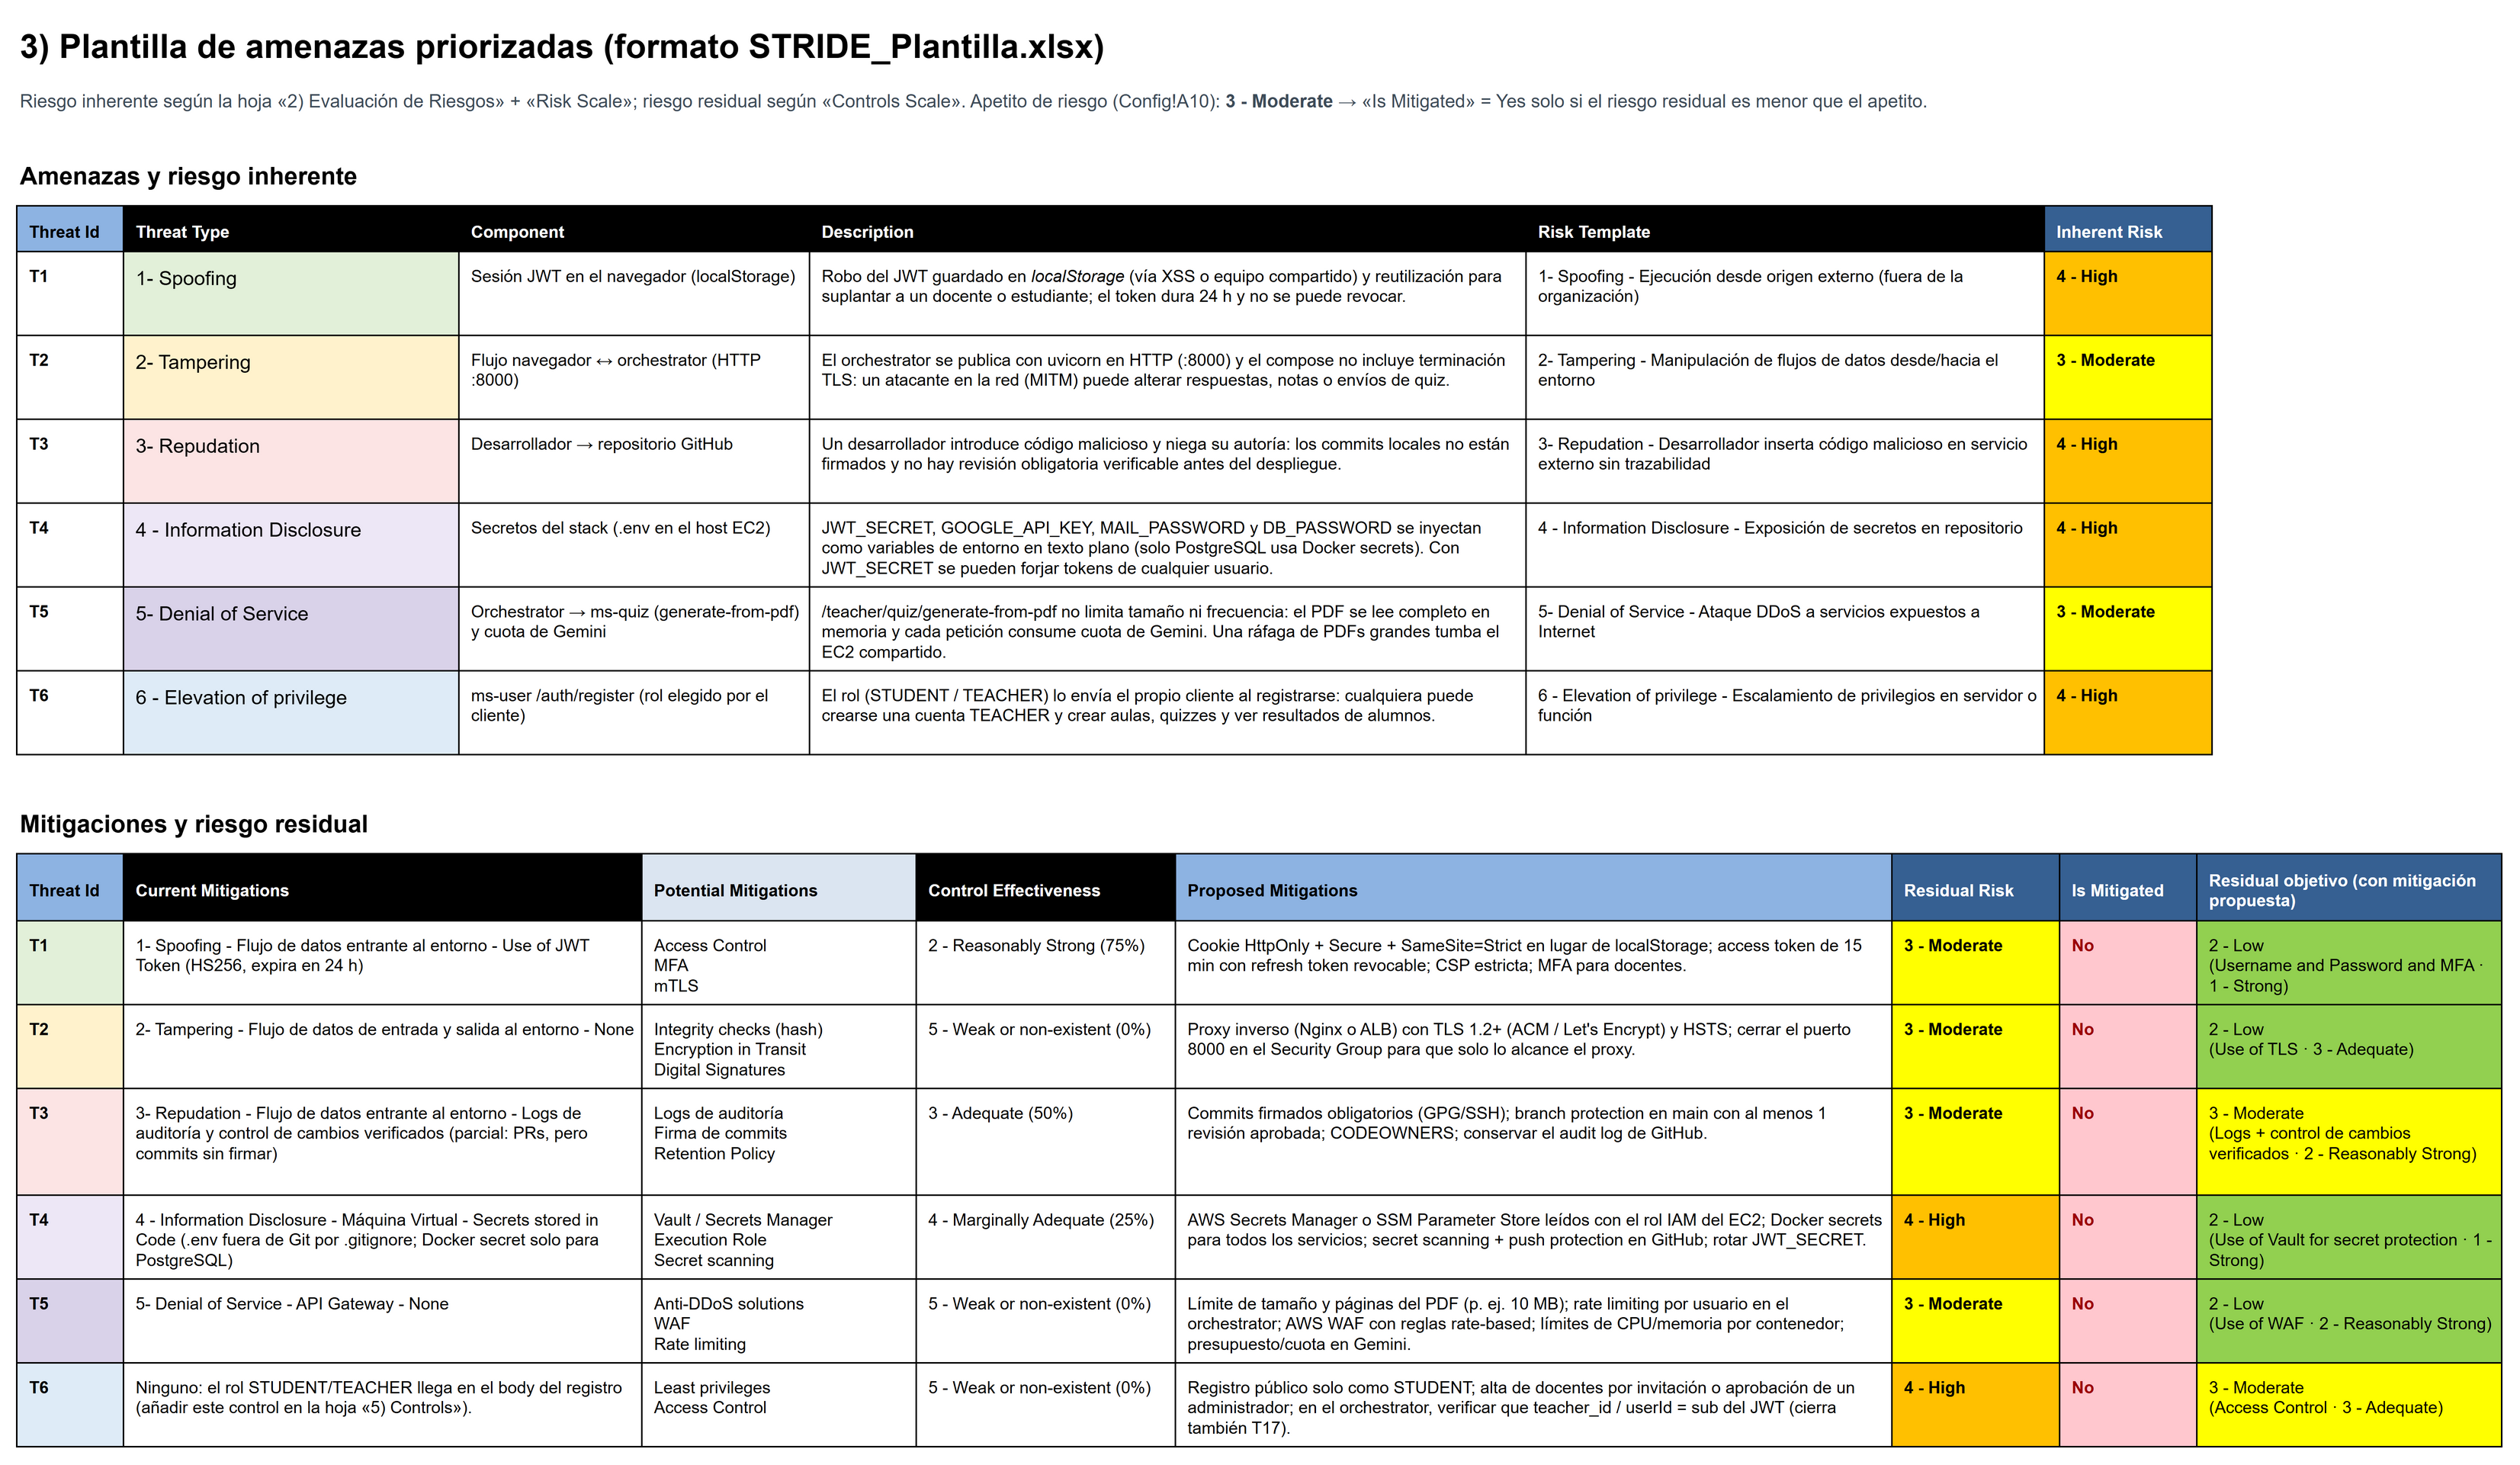
\includegraphics[width=\linewidth,height=0.80\textheight,keepaspectratio]{stride-plantilla.png}
  \caption{Hoja 3 del modelo: plantilla de amenazas priorizadas con riesgo inherente, mitigaciones
  actuales y propuestas, efectividad del control y riesgo residual.}
  \label{fig:stride-plantilla}
\end{figure}
\end{landscape}

\subsection{T1. Spoofing: sesión JWT en el navegador}

El frontend guarda el token en \texttt{localStorage} (\ruta{frontend/src/lib/api.ts}, líneas
49--69). Cualquier script que se ejecute en la página puede leerlo, y el token sigue siendo válido
durante 24 horas aunque el usuario cierre sesión. Un XSS o un equipo compartido, frecuente en el
contexto de la Sección~\ref{sec:justificacion}, bastan para suplantar a un docente o estudiante.
En el cierre se rotó \texttt{JWT\_SECRET} en la computadora revisada: un token anterior devuelve 401
y un login nuevo funciona. La amenaza sigue \textbf{pendiente}: hay que mover el token a una cookie
HttpOnly, Secure y SameSite, acortar su vigencia con un refresh token revocable y exigir MFA a los
docentes.

\subsection{T2. Tampering: tráfico sin TLS hacia el gateway}

El orchestrator publica el puerto 8000 por HTTP y \ruta{compose.yml} no incluye terminación TLS.
Quien controle la red entre el navegador y el servidor puede leer el token o alterar notas,
respuestas y envíos de quiz. Sigue \textbf{pendiente}: se recomienda un proxy inverso con TLS 1.2
o superior y HSTS, y cerrar el puerto 8000 al exterior para que solo el proxy lo alcance.

\subsection{T3. Repudiation: cambios sin firma}

Los Pull Requests dejan trazabilidad del código integrado, pero los commits no están firmados y la
revisión no es obligatoria. Un cambio malicioso podría atribuirse a otra persona o negarse. Sigue
\textbf{pendiente}: firma GPG o SSH obligatoria, protección de \texttt{main} con al menos una
aprobación y CODEOWNERS.

\subsection{T4. Information Disclosure: secretos del stack}

Solo la contraseña de PostgreSQL usa Docker secrets. \texttt{JWT\_SECRET},
\texttt{GOOGLE\_API\_KEY} y \texttt{MAIL\_PASSWORD} llegan a los contenedores como variables de
entorno. Además, Gitleaks detectó JWT en colecciones Bruno versionadas. El equipo sustituyó los
valores del árbol actual por variables, pero Gitleaks aún encuentra 46 ocurrencias en el historial,
que no se reescribió. El estado es \textbf{parcial}: falta un gestor de secretos (AWS Secrets
Manager o SSM) y confirmar la rotación de la clave en todas las computadoras del equipo.

\subsection{T5. Denial of Service: PDF y cuota de IA}

La generación desde PDF leía archivos sin límite y usaba una dependencia de lectura vulnerable. El
equipo migró a \texttt{pypdf} y ms-quiz rechaza archivos de más de 5~MB o de más de 30 páginas
(\ruta{ms-quiz/config/settings.py}); seis pruebas cubren esos límites. El estado es
\textbf{parcial}: falta limitar la frecuencia por usuario y la cuota de Gemini.

\subsection{T6. Elevation of Privilege: registro con rol docente}

El registro aceptaba el rol que enviaba el cliente. Ahora ms-user solo crea docentes con un código
de invitación (\texttt{TEACHER\_INVITE\_CODE}); si la variable está vacía, el registro docente queda
deshabilitado y el rol ADMIN no se puede autoasignar. Las pruebas de integración y el E2E comprueban
un 403 sin código válido. La amenaza está \textbf{mitigada}; la custodia del código es una tarea
operativa. La amenaza relacionada T17 (IDOR) también está mitigada en las rutas corregidas: el
gateway compara el usuario del token con el identificador recibido y responde 403 ante IDs ajenos.

\section{Análisis estático y dinámico: SAST y DAST}
\label{sec:sast-dast}

\subsection{Herramientas y configuración}

El pipeline ejecuta el análisis estático (SAST) en el job \texttt{sast}. \textbf{Semgrep} revisa
patrones inseguros en Python, JavaScript, TypeScript, Java y Dockerfiles, y \textbf{Bandit}
complementa el análisis de los servicios Python. Ambos generan reportes JSON que se conservan como
artefactos del run. \textbf{SonarCloud} está configurado en un job opcional e independiente, pero el
repositorio no tiene el secreto \texttt{SONAR\_TOKEN}: el job termina en verde sin ejecutar el
análisis, por lo que no se presenta como evidencia.

El análisis dinámico (DAST) corre en el job \texttt{dast}. Levanta un staging efímero con Docker
Compose sobre las imágenes recién construidas, registra un docente con código de invitación y pasa
su token a \textbf{OWASP ZAP}. ZAP ejecuta un \emph{API scan} contra la especificación OpenAPI del
gateway y un \emph{baseline scan} del frontend. Si no obtiene el token, el job falla: se eliminó el
recurso que antes continuaba en silencio con un análisis sin autenticación.

\subsection{Resultados}

La Tabla~\ref{tab:sast-dast} compara la línea base oficial (run 44965126475) con el corte de cierre
(run 45067822680). Los conteos de ZAP son alertas agrupadas por regla, no peticiones HTTP
individuales.

\begin{table}[htbp]
  \centering
  \caption{Detecciones de SAST y DAST en la línea base y en el cierre.}
  \label{tab:sast-dast}
  \small
  \begin{tabularx}{\textwidth}{llccY}
    \toprule
    \textbf{Herramienta} & \textbf{Tipo} & \textbf{Inicial} & \textbf{Cierre} &
    \textbf{Interpretación} \\
    \midrule
    Semgrep & SAST & 49 & 1 & Desaparecen los tokens del árbol y los patrones corregidos \\
    Bandit & SAST & 12 & 12 & Persisten hallazgos que requieren triage, como el binding a
    \texttt{0.0.0.0} dentro del contenedor (riesgo aceptado) \\
    OWASP ZAP & DAST & 22 & 16 & La línea base no autenticó; el cierre analiza la API con sesión \\
    \bottomrule
  \end{tabularx}
\end{table}

El valor del DAST autenticado se comprobó en el run 44966862163. Con sesión, ZAP detectó que el
perfil devolvía el hash BCrypt de la contraseña (regla 10097, hallazgo HIGH-005), algo que el
análisis sin sesión no podía ver. Tras excluir la contraseña de las respuestas, la alerta ya no
aparece en el reporte autenticado del cierre. Los reportes JSON de la línea base están en
\ruta{docs/devsecops/baseline}, y los de cada run, en sus artefactos de GitHub Actions.

\begin{figure}[htbp]
  \centering
  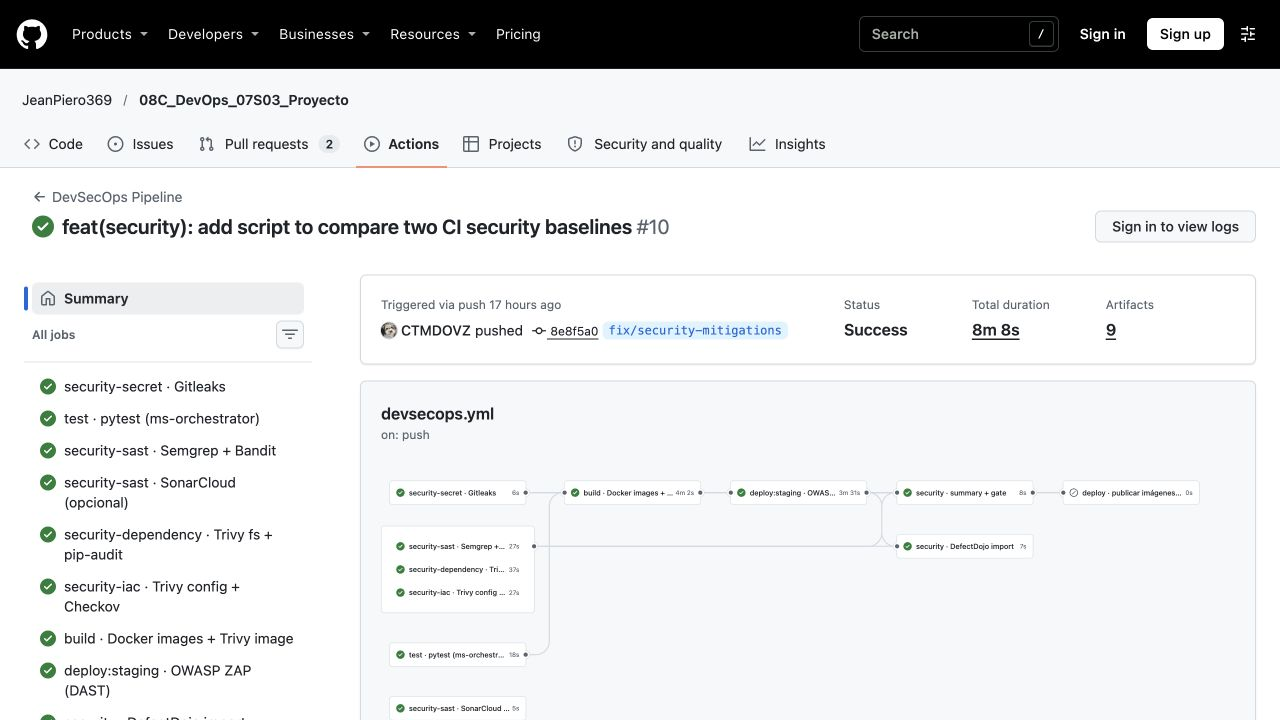
\includegraphics[width=0.95\textwidth]{github-run-historico.png}
  \caption{Ejecución del pipeline durante las mitigaciones (rama \texttt{fix/security-mitigations},
  commit 8e8f5a0): Gitleaks, pytest, Semgrep y Bandit, SonarCloud opcional, SCA, IaC, build, DAST,
  DefectDojo y gate terminan correctamente.}
  \label{fig:run-mitigaciones}
\end{figure}

\section{Secret scanning y análisis de dependencias}
\label{sec:sca}

\textbf{Gitleaks} revisa el historial completo del repositorio con redacción de valores en el job
\texttt{secret-scan}. \textbf{Trivy} analiza las dependencias del sistema de archivos (job
\texttt{sca}), la configuración de Dockerfiles y Compose (job \texttt{iac-scan}) y las imágenes de
los cinco servicios (job \texttt{build}). \textbf{pip-audit} revisa las dependencias declaradas de
Python y \textbf{Checkov} complementa la revisión de infraestructura como código. Un resumen
normaliza las severidades de todos los reportes.

\begin{table}[htbp]
  \centering
  \caption{Detecciones de secret scanning, SCA e IaC en la línea base y en el cierre.}
  \label{tab:sca}
  \small
  \begin{tabularx}{\textwidth}{lccY}
    \toprule
    \textbf{Herramienta} & \textbf{Inicial} & \textbf{Cierre} & \textbf{Interpretación} \\
    \midrule
    Gitleaks & 48 & 46 & Los JWT se retiraron del árbol actual; quedan 46 ocurrencias en el
    historial, que no se reescribió \\
    Trivy & 1063 & 597 & Actualización de Next.js, Spring Boot, dependencias de Node e imágenes
    base; el resto requiere triage \\
    pip-audit & 1 & 0 & PyPDF2 vulnerable reemplazado por \texttt{pypdf} \\
    Checkov & 3 & 0 & Se añadió HEALTHCHECK a los Dockerfiles de frontend, ms-classroom y
    ms-user \\
    \bottomrule
  \end{tabularx}
\end{table}

Estos números no se suman como vulnerabilidades únicas: un mismo aviso puede aparecer en el
análisis del sistema de archivos y en el de la imagen, o en varias imágenes. El propio pipeline
también se protegió contra la cadena de suministro: las acciones de terceros están fijadas por SHA
y los scripts verifican el checksum al descargar Gitleaks y Trivy. Persisten tags mutables en
algunas imágenes y reglas externas de los escáneres, por lo que la reproducibilidad es parcial.

\section{Centralización en DefectDojo}
\label{sec:defectdojo}

Se levantó una instancia propia de DefectDojo (\texttt{localhost:8080}) con el producto
\emph{Kiwi} y el engagement \emph{CI/CD main}. Primero se importaron los 15 reportes de la línea
base, uno por herramienta y objetivo. Después se reimportaron sobre los mismos tests los runs
44972251652 y 45067822680: al reimportar, DefectDojo marca como mitigados los hallazgos que ya no
aparecen y agrega los nuevos, lo que da el historial de cada hallazgo. Los 15 tests conservaron sus
identificadores.

\begin{table}[htbp]
  \centering
  \caption{Hallazgos activos en DefectDojo antes y después de las mitigaciones.}
  \label{tab:defectdojo}
  \small
  \begin{tabular}{lcccccc}
    \toprule
    \textbf{Estado} & \textbf{Critical} & \textbf{High} & \textbf{Medium} & \textbf{Low} &
    \textbf{Info} & \textbf{Total} \\
    \midrule
    Línea base importada & 33 & 381 & 485 & 276 & 22 & 1197 \\
    Cierre (activos) & 0 & 156 & 286 & 195 & 35 & 672 \\
    \bottomrule
  \end{tabular}
\end{table}

Tras todas las importaciones, la instancia registra 1233 hallazgos históricos: 672 activos y 561
mitigados; las reimportaciones crearon 36 registros nuevos. Las pequeñas diferencias en LOW e INFO
frente al resumen del CI se deben al parser de DefectDojo. Las propuestas de aceptación de riesgo
quedan pendientes de decisión del equipo.

El job \texttt{defectdojo} del pipeline puede reimportar automáticamente cada run, pero necesita la
URL y el token de una instancia accesible desde GitHub. Como esos secretos no están configurados, el
job no importa nada; la centralización mostrada se hizo en la instancia local con los mismos
artefactos del CI.

\begin{figure}[htbp]
  \centering
  \begin{subfigure}[t]{0.44\textwidth}
    \centering
    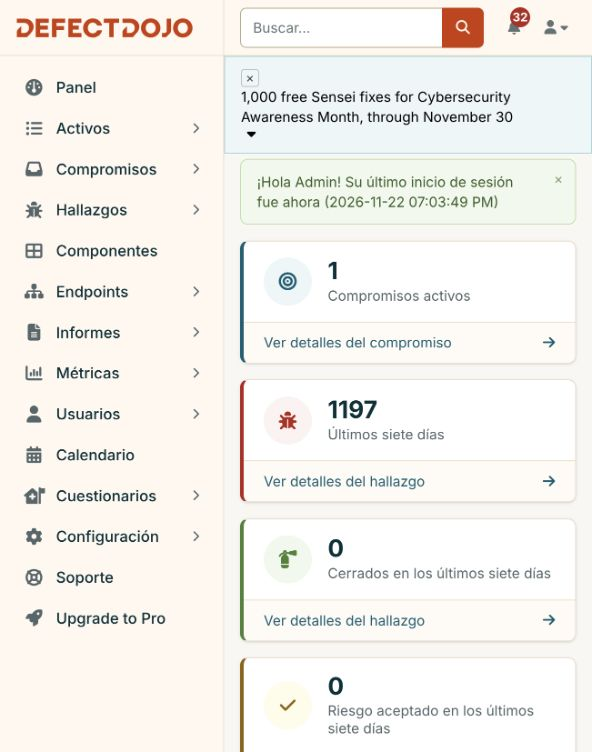
\includegraphics[width=\linewidth]{defectdojo-antes.png}
    \caption{Tras importar la línea base: 1197 hallazgos.}
  \end{subfigure}\hfill
  \begin{subfigure}[t]{0.52\textwidth}
    \centering
    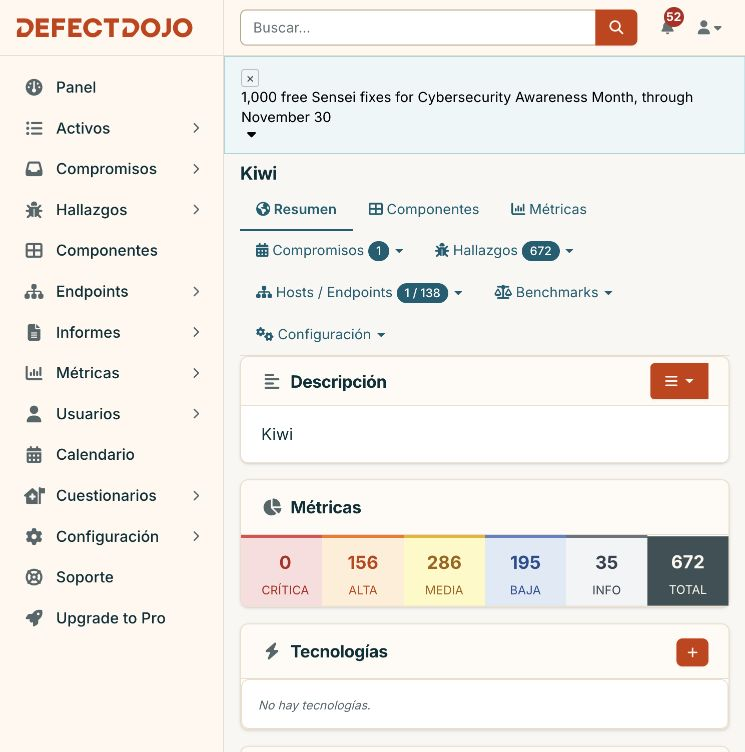
\includegraphics[width=\linewidth]{defectdojo-cierre.png}
    \caption{Producto Kiwi tras reimportar el cierre: 0 críticos y 672 activos.}
  \end{subfigure}
  \caption{Capturas de la instancia propia de DefectDojo.}
  \label{fig:defectdojo}
\end{figure}

\section{Tabla de mitigaciones}
\label{sec:mitigaciones}

La Tabla~\ref{tab:mitigaciones} prioriza por severidad ocho hallazgos del Excel del equipo, que
conserva las 20 filas originales con su estado. Entre paréntesis se indica la amenaza STRIDE
relacionada del modelo de la Sección~\ref{sec:stride}. Los hallazgos de revisión manual se
atribuyen a la revisión STRIDE y no a un escáner que no los detectó.

{\small\setlength{\tabcolsep}{4pt}
\begin{longtable}{L{1.9cm}L{3.2cm}L{1.9cm}L{2.4cm}L{4.8cm}}
  \caption{Hallazgos priorizados, recomendación y estado.}\label{tab:mitigaciones}\\
  \toprule
  \textbf{ID} & \textbf{Descripción} & \textbf{Severidad} & \textbf{Herramienta} &
  \textbf{Recomendación y estado} \\
  \midrule
  \endfirsthead
  \toprule
  \textbf{ID} & \textbf{Descripción} & \textbf{Severidad} & \textbf{Herramienta} &
  \textbf{Recomendación y estado} \\
  \midrule
  \endhead
  \bottomrule
  \endfoot
  CRIT-001 & Next.js 15.3.3 con ejecución remota de código no autenticada (React Flight) &
  CRITICAL & Trivy, npm audit & Actualizar Next.js y reconstruir la imagen. \textbf{Mitigado}:
  los avisos de la línea base no aparecen en el reporte posterior. \\
  \addlinespace
  CRIT-005 & Tomcat embebido y Spring desactualizados en ms-user & CRITICAL & Trivy image &
  Migrar a Spring Boot 4.0.10 (Tomcat 11.0.27, Spring 7.0.11). \textbf{Mitigado}: sin los
  CRITICAL anteriores. \\
  \addlinespace
  HIGH-001 (T4) & JWT versionados en colecciones Bruno & HIGH & Gitleaks, Semgrep & Sustituir por
  variables y rotar \texttt{JWT\_SECRET} en todos los entornos. \textbf{Parcial}: árbol limpio,
  46 ocurrencias históricas y rotación local verificada. \\
  \addlinespace
  HIGH-003 (T17) & IDs ajenos aceptados en compras e intentos (IDOR) & HIGH & Revisión STRIDE &
  Tomar la identidad del token y responder 403. \textbf{Mitigado} en las rutas cubiertas. \\
  \addlinespace
  HIGH-004 (T6) & Rol docente elegido por el cliente al registrarse & HIGH & Revisión STRIDE &
  Código de invitación validado por el servidor. \textbf{Mitigado} y comprobado con E2E. \\
  \addlinespace
  HIGH-005 & Hash BCrypt expuesto en la respuesta de perfil & HIGH & OWASP ZAP autenticado &
  Excluir la contraseña de las respuestas. \textbf{Mitigado} y comprobado con E2E. \\
  \addlinespace
  MED-002 (T5) & PyPDF2 vulnerable y lectura de PDF sin límites & MEDIUM & pip-audit & Migrar a
  \texttt{pypdf} y limitar tamaño y páginas. \textbf{Dependencia mitigada}; faltan cuota de IA y
  rate limiting. \\
  \addlinespace
  LOW-001 & Imágenes sin HEALTHCHECK & LOW & Checkov, Trivy config & Agregar HEALTHCHECK.
  \textbf{Mitigado}: seis servicios healthy. \\
\end{longtable}
}

\section{Situación inicial y resultados}
\label{sec:resultados}

\subsection{Antes y después de aplicar DevSecOps}

Antes del pipeline, el proyecto tenía pruebas unitarias y contenedores, pero ningún control de
seguridad automático: dependencias vulnerables, JWT versionados y errores de autorización podían
llegar a \texttt{main} sin que nadie los evaluara en conjunto. La línea base oficial (run
44965126475) registró 1198 detecciones, 33 de ellas CRITICAL. El corte de cierre (run 45067822680,
commit 41aaa61) registra 672 y ninguna CRITICAL.

\begin{table}[htbp]
  \centering
  \caption{Detecciones por severidad en la línea base y en el cierre.}
  \label{tab:antes-despues}
  \small
  \begin{tabular}{lccc}
    \toprule
    \textbf{Severidad} & \textbf{Inicial} & \textbf{Cierre} & \textbf{Reducción} \\
    \midrule
    CRITICAL & 33 & 0 & 100,0\,\% \\
    HIGH & 382 & 156 & 59,2\,\% \\
    MEDIUM & 485 & 286 & 41,0\,\% \\
    LOW & 275 & 194 & 29,5\,\% \\
    INFO & 23 & 36 & $-56{,}5$\,\% \\
    \midrule
    \textbf{Total} & \textbf{1198} & \textbf{672} & \textbf{43,9\,\%} \\
    CRITICAL y HIGH & 415 & 156 & 62,4\,\% \\
    \bottomrule
  \end{tabular}
\end{table}

Los totales se reprodujeron procesando los artefactos descargados de GitHub, con verificación de
hashes. Las dos mediciones no tienen exactamente la misma cobertura: el ZAP inicial no autenticó y
el de cierre sí, y las bases de vulnerabilidades, imágenes y dependencias cambian entre ejecuciones.
Por eso el porcentaje describe detecciones observadas, no una reducción exacta del riesgo ni del
número de vulnerabilidades únicas. INFO sube porque también agrupa avisos UNKNOWN de Trivy, que
requieren triage.

El cambio con más efecto fue migrar ms-user de Spring Boot 3.5.16 a 4.0.10, con Spring Framework
7.0.11, Tomcat 11.0.27 y PostgreSQL JDBC 42.7.14 administrados por su BOM. Se adaptaron los
matchers y constructores de Spring Security y se conservó el formato JSON con la opción de
compatibilidad de Jackson 3. Los avisos CVE-2026-47884 y CVE-2026-47890 ya no aparecen. No se
introdujeron exclusiones ni se rebajó el umbral del gate para conseguir el resultado.

\subsection{Confirmación en la rama principal}

Tras integrar los Pull Requests \#11, \#12 y \#13, el pipeline se ejecutó sobre \texttt{main} (run
45104881204, commit cf0e932) con el mismo resultado: 672 detecciones y ninguna CRITICAL. La
Tabla~\ref{tab:main-herramientas} desglosa ese resultado por herramienta; pip-audit y Checkov no
aparecen porque no reportan hallazgos.

\begin{table}[htbp]
  \centering
  \caption{Detecciones por herramienta en el run de \texttt{main} 45104881204.}
  \label{tab:main-herramientas}
  \small
  \begin{tabular}{lcccccc}
    \toprule
    \textbf{Herramienta} & \textbf{Critical} & \textbf{High} & \textbf{Medium} & \textbf{Low} &
    \textbf{Info} & \textbf{Total} \\
    \midrule
    Bandit & 0 & 0 & 2 & 10 & 0 & 12 \\
    Gitleaks & 0 & 46 & 0 & 0 & 0 & 46 \\
    OWASP ZAP & 0 & 0 & 3 & 6 & 7 & 16 \\
    Semgrep & 0 & 0 & 0 & 0 & 1 & 1 \\
    Trivy & 0 & 110 & 281 & 178 & 28 & 597 \\
    \midrule
    \textbf{Total} & \textbf{0} & \textbf{156} & \textbf{286} & \textbf{194} & \textbf{36} &
    \textbf{672} \\
    \bottomrule
  \end{tabular}
\end{table}

\section{Pipeline CI/CD completo}
\label{sec:pipeline}

\subsection{Estructura}

El workflow \ruta{.github/workflows/devsecops.yml} se ejecuta en cada push a \texttt{main},
\texttt{feat/**} y \texttt{fix/**}, en los Pull Requests hacia \texttt{main} y de forma manual.
Declara 12 jobs (Tabla~\ref{tab:jobs}). Los análisis y las pruebas corren en paralelo; el build
espera a las pruebas de Python y al secret scanning; el DAST espera al build; el gate consolida todos
los reportes, y la publicación de imágenes solo ocurre en un push a \texttt{main} cuando todo lo
anterior terminó bien. La Figura~\ref{fig:pipeline} muestra las dependencias y el Anexo~\ref{sec:anexo-yaml}
reproduce la configuración completa.

\begin{table}[htbp]
  \centering
  \caption{Jobs del pipeline DevSecOps.}
  \label{tab:jobs}
  \small
  \begin{tabularx}{\textwidth}{L{3.1cm}L{4.6cm}Y}
  \toprule
  \textbf{Job} & \textbf{Herramientas} & \textbf{Depende de y condición} \\
  \midrule
  \texttt{secret-scan} & Gitleaks & Ninguno \\
  \texttt{unit-tests} & pytest (gateway y ms-quiz) & Ninguno \\
  \texttt{java-unit-tests} & JUnit, Java 17, Testcontainers & Ninguno \\
  \texttt{sast} & Semgrep y Bandit & Ninguno \\
  \texttt{sonarcloud} & SonarCloud (opcional) & Ninguno; requiere \texttt{SONAR\_TOKEN} \\
  \texttt{sca} & Trivy fs y pip-audit & Ninguno \\
  \texttt{iac-scan} & Trivy config y Checkov & Ninguno \\
  \texttt{build} & Docker build de 5 imágenes y Trivy image & \texttt{unit-tests},
  \texttt{secret-scan} \\
  \texttt{dast} & Staging con Compose, OWASP ZAP autenticado y sondas & \texttt{build} \\
  \texttt{defectdojo} & Reimportación de reportes (opcional) & Escaneos y DAST; no se ejecuta en
  Pull Requests \\
  \texttt{security-gate} & Resumen de 15 reportes y umbral & Escaneos y DAST; se ejecuta siempre \\
  \texttt{release} & Publicación en GHCR & Gate, pruebas, escaneos, build y DAST; solo push a
  \texttt{main} \\
  \bottomrule
  \end{tabularx}
\end{table}

\begin{figure}[htbp]
  \centering
  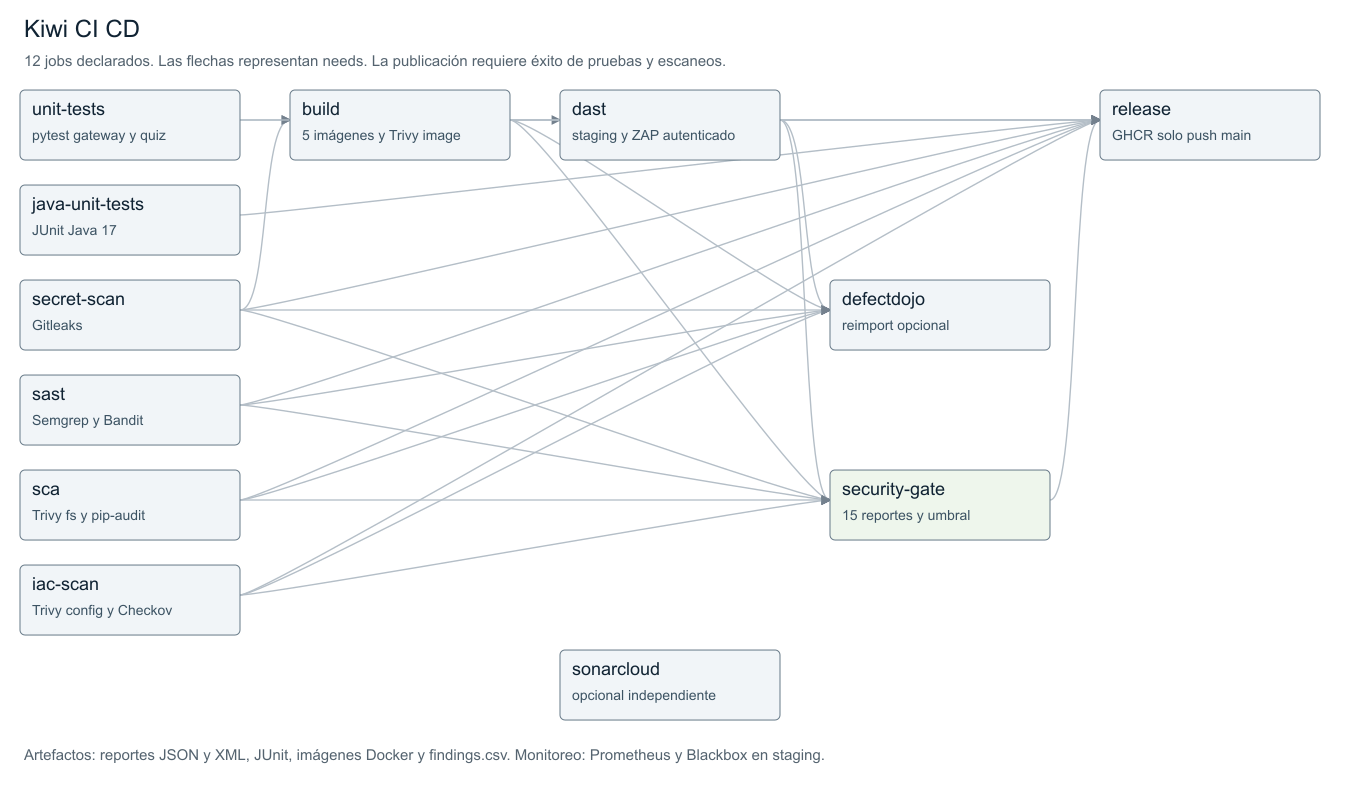
\includegraphics[width=\textwidth]{pipeline-grafo.png}
  \caption{Dependencias (\texttt{needs}) entre los 12 jobs del pipeline. La publicación requiere el
  éxito de pruebas, escaneos, build, DAST y gate.}
  \label{fig:pipeline}
\end{figure}

\subsection{Gate de seguridad}

El job \texttt{security-gate} exige los 15 reportes JSON esperados; si falta alguno o no se puede
leer, falla, de modo que una herramienta que no se ejecutó no pasa por éxito. Luego consolida las
severidades en un resumen y un CSV, y bloquea el pipeline si encuentra hallazgos iguales o
superiores al umbral. El umbral por defecto es CRITICAL y la variable
\texttt{SECURITY\_GATE\_SEVERITY} permite endurecerlo a HIGH. En el run 45067822680 el gate
verificó los 15 reportes sin errores y aprobó con cero CRITICAL; el release se omitió porque la
rama no era \texttt{main} (Figura~\ref{fig:run-cierre}).

\begin{figure}[htbp]
  \centering
  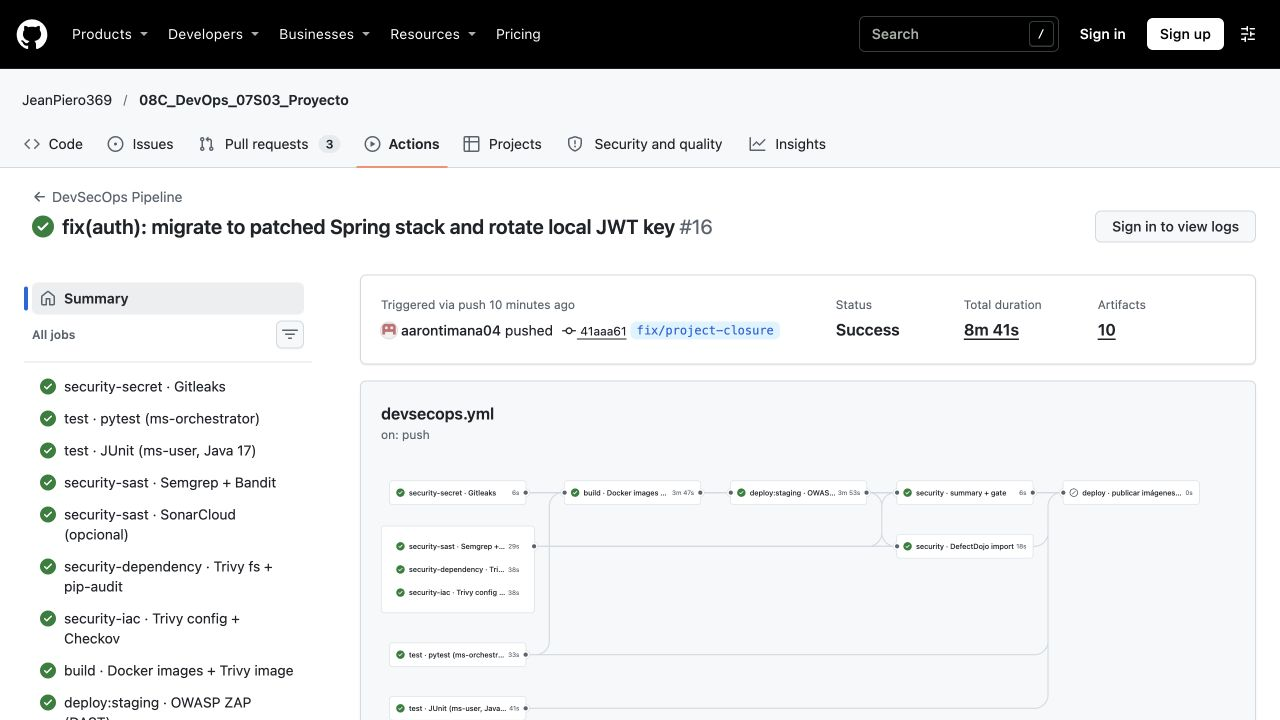
\includegraphics[width=0.95\textwidth]{github-run-cierre.png}
  \caption{Run 45067822680 de la rama \texttt{fix/project-closure}: pruebas, análisis, staging y
  gate correctos; publicación omitida fuera de \texttt{main}.}
  \label{fig:run-cierre}
\end{figure}

En \texttt{main} (run 45104881204) los once jobs previos terminaron correctamente y el release se
ejecutó por primera vez. Publicó en GHCR las imágenes de ms-user, ms-classroom, ms-quiz y
orchestrator, etiquetadas con el commit, pero el registro rechazó la de frontend con un error
\texttt{denied}, por lo que el run figura como fallido. El error apunta a los permisos del paquete
\texttt{kiwi-frontend} en GHCR, no al código ni a los controles de seguridad, y queda como pendiente
(Sección~\ref{sec:recomendaciones}).

\section{Ambientes y monitoreo}
\label{sec:ambientes}

\subsection{Ambientes}

La Tabla~\ref{tab:ambientes} resume los ambientes y lo que se validó en cada uno. El mismo
\ruta{compose.yml} se usa en desarrollo y en el staging de CI, con credenciales distintas: el
staging crea variables efímeras en cada ejecución (\ruta{security/scripts/ci_env.sh}) y usa datos
ficticios.

\begin{table}[htbp]
  \centering
  \caption{Ambientes del proyecto.}
  \label{tab:ambientes}
  \small
  \begin{tabularx}{\textwidth}{L{2.6cm}YY}
    \toprule
    \textbf{Ambiente} & \textbf{Ejecución y datos} & \textbf{Validación} \\
    \midrule
    Desarrollo & Docker Compose local con credenciales propias y datos ficticios & Pruebas
    unitarias y 16 comprobaciones E2E \\
    \addlinespace
    Staging (CI) & Compose efímero sobre las imágenes construidas en el run & ZAP autenticado,
    sondas HTTP y reportes \\
    \addlinespace
    Distribución & Job \texttt{release} hacia GHCR en cada push a \texttt{main} & Ejecutado en el
    run 45104881204: cuatro de cinco imágenes publicadas \\
    \addlinespace
    Producción & Arquitectura objetivo: frontend en AWS Amplify y backend con Compose en AWS EC2 &
    Sin despliegue automatizado ni operación acreditada en este informe \\
    \bottomrule
  \end{tabularx}
\end{table}

\subsection{Monitoreo}

El archivo \ruta{compose.monitoring.yml} añade \textbf{Prometheus} y \textbf{Blackbox Exporter}.
Dos sondas consultan cada 15 segundos el frontend y la especificación OpenAPI del gateway.
\texttt{probe\_success} indica si el servicio responde por HTTP y \texttt{probe\_duration\_seconds}
mide la duración de la sonda. Dos alertas completan la configuración: \texttt{KiwiEndpointDown},
cuando un servicio deja de responder, y \texttt{KiwiProbeMissing}, cuando Prometheus deja de
recibir la métrica. Los healthchecks de Compose vigilan además el estado de cada contenedor.

La configuración y las reglas se validaron con \texttt{promtool}. En una prueba controlada se
detuvo el frontend, se observó \texttt{KiwiEndpointDown} en estado \emph{firing} tras el período
definido, se restauró el servicio y se comprobó que la alerta desaparecía con las dos sondas de
nuevo sanas. El job \texttt{dast} ejecuta las mismas sondas sobre el staging de CI. No se
configuraron notificaciones externas, y estas señales no reemplazan métricas de negocio ni
pruebas de carga.

\begin{figure}[htbp]
  \centering
  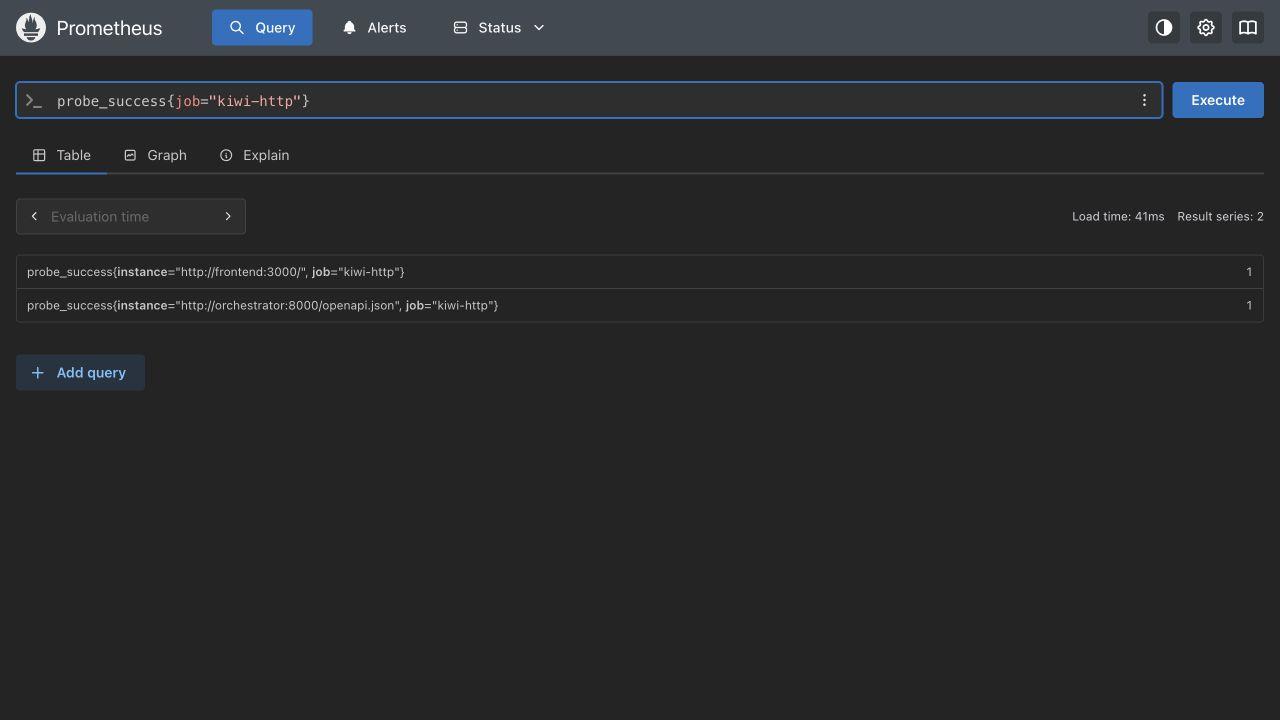
\includegraphics[width=0.9\textwidth]{prometheus-sondas.png}
  \caption{Prometheus con las dos sondas HTTP de KIWI en estado correcto
  (\texttt{probe\_success} = 1). Las evidencias JSON conservan la caída, la alerta y la
  recuperación.}
  \label{fig:prometheus}
\end{figure}

\section{Modelo de madurez}
\label{sec:madurez}

Se usa OWASP SAMM 2 como modelo de madurez de seguridad dentro de DevSecOps. SAMM organiza cinco
funciones de negocio (gobierno, diseño, implementación, verificación y operaciones) en quince
prácticas, cada una con tres niveles. La Tabla~\ref{tab:samm} es una autoevaluación del proyecto
académico sobre las prácticas que el trabajo tocó; no es una certificación ni una puntuación global.

\begin{table}[htbp]
  \centering
  \caption{Autoevaluación OWASP SAMM de las prácticas trabajadas.}
  \label{tab:samm}
  \small
  \begin{tabularx}{\textwidth}{L{3.0cm}YY}
    \toprule
    \textbf{Práctica SAMM} & \textbf{Evidencia} & \textbf{Situación alcanzada} \\
    \midrule
    Threat Assessment & DFD y STRIDE con 17 amenazas, seis evaluadas con la plantilla & Actividades
    iniciales documentadas \\
    \addlinespace
    Secure Build & Build automatizado, acciones fijadas por SHA y análisis de dependencias &
    Automatización implementada, reproducibilidad parcial \\
    \addlinespace
    Defect Management & DefectDojo con reimportación y estados por hallazgo & Seguimiento inicial
    operativo \\
    \addlinespace
    Security Testing & SAST, DAST autenticado y pruebas negativas de controles & Objetivo del
    nivel 1 demostrado en el alcance revisado \\
    \addlinespace
    Incident Management & Sondas, alertas y prueba de caída y recuperación & Detección básica,
    sin proceso de respuesta ni operación productiva \\
    \bottomrule
  \end{tabularx}
\end{table}

El nivel 1 de Security Testing consiste en descubrir defectos con herramientas automáticas y pruebas
manuales; el proyecto aporta ambos tipos de evidencia y automatiza parte de ellos en CI. No se
declara un nivel 2 o 3 global: faltan la evaluación completa de cada práctica, pruebas de
penetración periódicas, acuerdos operativos, rotación confirmada de claves y mediciones sostenidas.

\section{Lecciones aprendidas}
\label{sec:lecciones}

\subsection{Problema de negocio que resuelve el proyecto}

KIWI ofrece refuerzo de Comunicación a estudiantes de primero de secundaria con acceso limitado a
dispositivos (Sección~\ref{sec:justificacion}). Para la institución, el sistema solo es útil si es
confiable: guarda identidades, resultados y recompensas de menores de edad, y permite a los docentes
evaluar. Una cuenta docente falsa, una nota alterada o un token robado afectan directamente la
confianza de docentes y familias.

\subsection{Limitaciones antes de aplicar DevOps}

Al inicio, cada microservicio se construía y probaba a mano con su propio stack. No había un punto
que verificara el sistema completo, y los errores aparecían al integrar: una dependencia del
frontend llegaba de forma indirecta por otro paquete y dependencias Python sin fijar rompieron el
arranque. La seguridad no se evaluaba: dependencias con avisos críticos, JWT versionados en
colecciones de prueba y un registro que aceptaba el rol enviado por el cliente pudieron entrar al
repositorio sin que nadie los detectara.

\subsection{Qué cambió con DevOps y DevSecOps}

Las ramas cortas con Pull Requests, Docker Compose y \texttt{kiwi.sh} hicieron reproducible el
entorno de los cinco componentes. El pipeline convirtió la seguridad en un
paso más de cada push: siete herramientas producen reportes comparables, el gate bloquea los
hallazgos críticos y DefectDojo registra qué se mitigó y cuándo. El modelo STRIDE dirigió la
revisión manual hacia rutas concretas, y así aparecieron fallos que ningún escáner reportaba, como
el registro docente y el IDOR. El DAST autenticado mostró, a su vez, la divulgación del hash que el
análisis sin sesión no veía.

También hubo lecciones sobre el propio pipeline. Una carrera de arranque de ms-user obligó a esperar
su disponibilidad antes de registrar el usuario de ZAP; convertir esa falla en un análisis sin
autenticación reducía la cobertura sin que el job fallara, por lo que se eliminó. Un job verde
tampoco garantiza un análisis: SonarCloud y la importación remota a DefectDojo terminan bien sin
credenciales. Por eso el gate exige los reportes en lugar de confiar en el color del job.

\subsection{Ventajas concretas}

\begin{itemize}[leftmargin=*]
  \item \textbf{Menos exposición medible}: de 33 detecciones CRITICAL a 0 y de 415 CRITICAL y
  HIGH a 156 (Tabla~\ref{tab:antes-despues}).
  \item \textbf{Controles verificables}: 53 pruebas automatizadas y 16 comprobaciones E2E
  confirman cada mitigación y detectan regresiones, como un PATCH de perfil que no reenviaba el
  cuerpo.
  \item \textbf{Trazabilidad}: cada cifra se asocia a un commit, un run y un reporte; DefectDojo
  conserva el estado de cada hallazgo entre ejecuciones.
  \item \textbf{Integración más segura}: ninguna imagen se publica si fallan las pruebas, los
  escaneos o el gate.
  \item \textbf{Detección temprana de caídas}: las sondas y la alerta comprobada avisan cuando un
  servicio deja de responder.
\end{itemize}

No se atribuyen mejoras de rendimiento, de aprendizaje de los estudiantes ni de disponibilidad
productiva, porque no se midieron.

\section{Recomendaciones}
\label{sec:recomendaciones}

\subsection{Para otros proyectos}

\begin{itemize}[leftmargin=*]
  \item Empezar por un inventario de servicios y un modelo de amenazas ligado a rutas concretas
  del código, y revisarlo cuando cambie la arquitectura.
  \item Escribir pruebas negativas que verifiquen qué ocurre cuando un usuario actúa sobre recursos
  ajenos o pide un rol que no le corresponde. Los escáneres no sustituyen esas pruebas.
  \item Hacer que el pipeline falle si una herramienta no produce su reporte, fijar umbrales
  explícitos y hacer depender la publicación de pruebas, escaneos y gate.
  \item Ejecutar el DAST con sesión: sin autenticación, gran parte de la API queda fuera del
  análisis.
  \item Registrar en cada evidencia el commit, el run, la versión de la herramienta y la cobertura,
  y hacer triage humano de los resultados antes de aceptar riesgos.
\end{itemize}

\subsection{Pendientes de KIWI}

\begin{itemize}[leftmargin=*]
  \item \textbf{T1}: mover el token a una cookie HttpOnly con vigencia corta y refresh token, y
  exigir MFA a los docentes.
  \item \textbf{T2}: poner un proxy con TLS y HSTS delante del gateway y cerrar el puerto 8000.
  \item \textbf{T3}: exigir commits firmados, protección de \texttt{main} con revisión aprobada y
  CODEOWNERS.
  \item \textbf{T4}: llevar los secretos a un gestor (AWS Secrets Manager o SSM), confirmar la
  rotación de \texttt{JWT\_SECRET} en todas las computadoras y decidir si se purga el historial.
  \item \textbf{T5}: limitar la frecuencia por usuario y la cuota de Gemini.
  \item \textbf{Pipeline}: corregir los permisos del paquete \texttt{kiwi-frontend} en GHCR y
  configurar \texttt{SONAR\_TOKEN} y una instancia de DefectDojo accesible desde CI.
  \item \textbf{Operación}: antes de atender usuarios reales, separar credenciales por ambiente,
  probar copias y restauración, ampliar la autorización por pertenencia a cada aula y asignar
  responsables al monitoreo.
\end{itemize}

\section{Conclusiones}

El uso de Conventional Commits y Pull Requests permite reconstruir el crecimiento del sistema y
distinguir funcionalidades, correcciones, infraestructura, pruebas y documentación. La estrategia
de ramas cortas mantiene a \texttt{main} como punto de integración y resulta coherente con Trunk
Based Development. Docker Compose, \texttt{kiwi.sh} y las pruebas unitarias dieron al equipo un
entorno reproducible sobre el que se construyó el resto.

El modelo STRIDE identificó 17 amenazas sobre siete fronteras de confianza y priorizó seis, una por
categoría. El pipeline de 12 jobs integra secret scanning, SAST, SCA, IaC, DAST autenticado, un gate
que exige reportes completos y la publicación condicionada en GHCR. Con esas herramientas y las
mitigaciones aplicadas, las detecciones bajaron de 1198 a 672 y las críticas de 33 a 0, resultado
confirmado en \texttt{main}. DefectDojo centraliza el historial de los hallazgos y Prometheus vigila
la disponibilidad con una alerta comprobada.

El proyecto queda en un nivel inicial de madurez: los controles de identidad del navegador, TLS,
firma de commits y gestión de secretos siguen pendientes, y no se acredita operación productiva. La
principal lección es que la seguridad funciona cuando se verifica en cada cambio: un modelo de
amenazas sin pruebas, o un pipeline verde sin reportes, dan una falsa sensación de control.

\clearpage
\appendix
\renewcommand{\thesection}{\Alph{section}}

\section{Configuración del pipeline}
\label{sec:anexo-yaml}

Copia de \ruta{.github/workflows/devsecops.yml}, idéntica a la versión integrada en \texttt{main}
salvo por los separadores decorativos de los comentarios, convertidos a guiones ASCII para la
tipografía del anexo.

\lstinputlisting[style=yaml,caption={Workflow \texttt{devsecops.yml} del pipeline DevSecOps.},label={lst:devsecops}]{devsecops.yml}

\section{Enlaces de entrega y referencias}
\label{sec:enlaces}

\subsection{Entregables}

\begin{itemize}[leftmargin=*]
  \item Repositorio:
  \url{https://github.com/JeanPiero369/08C_DevOps_07S03_Proyecto}
  \item Diagramas STRIDE (draw.io, hojas de arquitectura, amenazas y plantilla):
  \url{https://drive.google.com/file/d/1F9v70tKTnEiHMfKXY2khyDIHPxsQLHgG/view?usp=sharing}
  \item Copia del diagrama en el repositorio:
  \url{https://github.com/JeanPiero369/08C_DevOps_07S03_Proyecto/blob/main/docs/devsecops/stride/kiwi_stride.drawio}
  \item Excel STRIDE del equipo:
  \url{https://github.com/JeanPiero369/08C_DevOps_07S03_Proyecto/blob/main/docs/devsecops/stride/kiwi_stride.xlsx}
  \item Presentación:
  \url{https://github.com/JeanPiero369/08C_DevOps_07S03_Proyecto/blob/main/docs/devsecops/entrega/Kiwi_Presentacion_Final.pdf}
  \item Workflow del pipeline:
  \url{https://github.com/JeanPiero369/08C_DevOps_07S03_Proyecto/blob/main/.github/workflows/devsecops.yml}
\end{itemize}

\subsection{Evidencias de CI}

\begin{itemize}[leftmargin=*]
  \item Línea base oficial (run 44965126475):
  \url{https://github.com/JeanPiero369/08C_DevOps_07S03_Proyecto/actions/runs/44965126475}
  \item DAST autenticado adicional (run 44966862163):
  \url{https://github.com/JeanPiero369/08C_DevOps_07S03_Proyecto/actions/runs/44966862163}
  \item Resultado histórico (run 44972251652):
  \url{https://github.com/JeanPiero369/08C_DevOps_07S03_Proyecto/actions/runs/44972251652}
  \item Corte de cierre (run 45067822680):
  \url{https://github.com/JeanPiero369/08C_DevOps_07S03_Proyecto/actions/runs/45067822680}
  \item Rama principal tras el merge (run 45104881204):
  \url{https://github.com/JeanPiero369/08C_DevOps_07S03_Proyecto/actions/runs/45104881204}
  \item Pull Request de cierre (\#13):
  \url{https://github.com/JeanPiero369/08C_DevOps_07S03_Proyecto/pull/13}
\end{itemize}

\subsection{Referencias}

\begin{itemize}[leftmargin=*]
  \item Microsoft. \emph{STRIDE: modelado de amenazas}.
  \url{https://learn.microsoft.com/en-us/azure/security/develop/threat-modeling-tool-threats}
  \item OWASP. \emph{Software Assurance Maturity Model (SAMM)}.
  \url{https://owaspsamm.org/model/}
  \item OWASP SAMM. \emph{Security Testing}.
  \url{https://owaspsamm.org/model/verification/security-testing/}
  \item Prometheus. \emph{Understanding and using the multi-target exporter pattern}.
  \url{https://prometheus.io/docs/guides/multi-target-exporter/}
  \item Apache Tomcat. \emph{Security vulnerabilities fixed in Tomcat 11}.
  \url{https://tomcat.apache.org/security-11.html}
  \item Spring. \emph{CVE-2026-47884}. \url{https://spring.io/security/cve-2026-47884/}
  \item Spring. \emph{CVE-2026-47890}. \url{https://spring.io/security/cve-2026-47890/}
  \item Spring Boot. \emph{Spring Boot 4.0 Migration Guide}.
  \url{https://github.com/spring-projects/spring-boot/wiki/Spring-Boot-4.0-Migration-Guide}
\end{itemize}

\end{document}
